\documentclass[11pt,a4paper]{article}
\usepackage[margin=0.86in]{geometry}
\usepackage[T1]{fontenc}
\usepackage[utf8]{inputenc}
\usepackage{lmodern}
\usepackage{microtype}
\usepackage{amsmath,amssymb,booktabs,graphicx,tabularx,longtable,array}
\usepackage{caption,subcaption,float,enumitem,xcolor}
\usepackage[hidelinks]{hyperref}
\usepackage{siunitx}
\sisetup{detect-all}
\newcommand{\method}[1]{\texttt{#1}}
\newcommand{\BERT}{\ensuremath{\mathrm{BERTScore}_{F_1}}}
\newcommand{\ROUGE}{\ensuremath{\mathrm{ROUGE\mbox{-}L}_{F_1}}}
\newcommand{\ppl}{\ensuremath{\mathrm{PPL}}}
\title{Developing a Compact, Self-Hosted Legal Language Foundation:\\
Pretraining, Entity Recognition, Rhetorical Roles, Judgment Prediction, and Summarization}
\author{CS781 Legal Intelligence Capstone\\\small Master Research Report --- Phases 1--4 and 6}
\date{9 November 2026 --- working research edition}
\begin{document}
\maketitle
\begin{abstract}
This report documents the first phase of a sequential, self-hosted legal natural-language-processing capstone: the construction of a compact, from-scratch legal language model under an official-data-only constraint. We implemented and trained four architecturally different Transformer variants: a conventional causal decoder, an encoder--decoder, a prefix-language-model hybrid, and an efficient causal Transformer using grouped-query attention, rotary position embeddings, RMS normalization, and SwiGLU feed-forward layers. A custom 32,000-token byte-level BPE tokenizer was trained exclusively on the supplied corpus. At approximately 100 million pretraining tokens, the 112.679-million-parameter efficient grouped-query model attained the best official BERTScore F1 of \textbf{0.83479506} on 1,000 hidden-reference continuations. We then tokenized all four available legal sources (approximately 4.488 billion usable BPE tokens) and continued this model to 300, 500, and 700 million consumed tokens. Despite declining validation cross-entropy through 700 million tokens, all three continuation submissions scored below the original winner on the hidden test. A locally successful decoder selection at 500 million tokens likewise failed to improve official BERTScore. We present the corpus construction, architecture definitions, training and resume protocol, seven official submissions, quantitative local and private results, and the resulting lessons about validation objectives, decoding, model selection, and reproducible legal language generation. Phase 2 adapts these foundations to legal named entity recognition over 70 labeled judgments. Exact-span majority voting across two fully fine-tuned models and a distilled student attained the best official strict macro-F1, \textbf{0.3577}, after retraining on all labeled judgments. The original majority ensemble scored 0.3342. We report the adaptation controls, class imbalance, and error analysis alongside the separate local and official evaluations. Phase 3 studies sentence-level rhetorical roles and reaches official macro-F1 0.4249 using contextual Efficient GQA. Phase 4 compares eight trained classifiers and two blends for binary judgment prediction. Full Efficient GQA fine-tuning reaches the best recorded official macro-F1 of \textbf{0.7393}. Phase 6 investigates long-judgment summarization across three revisions. The submitted Efficient GQA LoRA model achieves the best recorded official BERTScore F1 of \textbf{0.8459}, while the gold-only causal student leads on held-out ROUGE.
\end{abstract}
\tableofcontents
\newpage

\section{Project Motivation and Scope}
Legal practice involves large amounts of sensitive natural-language material: judgments, statutes, party submissions, and potentially privileged client records. Sending confidential documents to a remote model endpoint is incompatible with the motivating deployment scenario. The capstone therefore investigates whether an entirely self-hosted language foundation can be trained and adapted within limited compute and model-size constraints. Phase 1 establishes that foundation, and Phase 2 adapts it to entity extraction. Later phases address rhetorical structure, judgment outcomes, statutory references, summarization, and prior-case retrieval.

The scientific question in Phase 1 is not simply whether a language model can imitate legal prose. It is which compact architecture and training/decoding decisions best support the exact continuation task, and whether improvements in next-token language-model fit also improve the hidden-reference continuation metric. The official evaluation takes a \emph{512-word legal prompt} and requires a \emph{128-word continuation} in a JSON field without repeating the prompt. Official Phase-1 ranking uses BERTScore F1, with ROUGE-L F1 and BLEU-4 as secondary metrics. The dataset provides no public test continuations; local evaluation instead uses held-out documents and internally constructed prompt--continuation examples.

\paragraph{Competition constraints.} The models must be trained from scratch using official data only; pretrained LMs, externally scraped legal corpora, commercial inference/training APIs, and models exceeding 300 million parameters are prohibited. The prescribed foundation size is 50--300 million parameters, and four \emph{substantially different} architectures must be investigated. The submission format is a ZIP containing \method{prediction.json} directly at the archive root. Each output has exactly the official example IDs and 128 words per continuation. This study focuses on the reproducible implementation and analysis of these obligations; it makes no claim of having performed a separate human legal-validity assessment.

\section{Phase 1: Data and Problem Formulation}
\subsection{Official dataset organization}
The course dataset \path{Exploration-Lab/CS-781-Capstone} provided all training data. We used its \path{Phase_1_Pretraining} configuration. Statutory acts and High Court judgments come from \path{train_acts.json} and \path{train_high_courts.json}. Supreme Court judgments and tribunal decisions come from \path{train_supreme_court.json} and \path{train_tribunals.json}. These sources differ in document structure, stylistic density, and abundance. The official \path{Test/test.json} contains 1,000 prompts with hidden continuation references.

\begin{table}[htbp]\centering\small
\caption{Full-corpus preprocessing results taken from the final executed notebook. Token quantities and weights shown here are rounded; counts are specific to the custom BPE tokenizer.}
\label{tab:corpus}
\begin{tabular}{lrrrr}
\toprule
Source & Train documents & Held-out documents & Train BPE tokens (B) & Mix probability \\
\midrule
Acts & 18,624 & 202 & 0.1535 & 0.0684 \\
High Courts & 2,511,473 & 25,265 & 2.4007 & 0.4688 \\
Supreme Court & 55,017 & 532 & 0.2579 & 0.0983 \\
Tribunals & 860,490 & 8,642 & 1.6760 & 0.3645 \\
\midrule
Total & 3,445,604 & 34,641 & \textbf{4.4881} & 1.0000 \\
\bottomrule
\end{tabular}
\end{table}

\begin{figure}[htbp]\centering
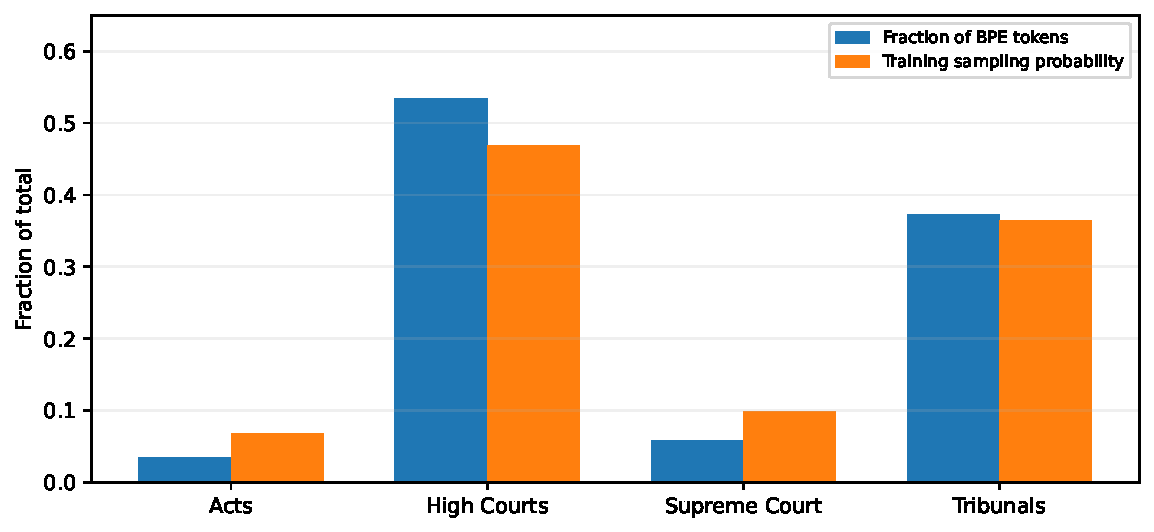
\includegraphics[width=.82\linewidth]{figures/phase1/p1_corpus_mixing.pdf}
\caption{Source abundance and subsequent temperature-balanced sampling probability. Sampling raises the relative contribution of smaller legal sources without discarding large sources.}
\label{fig:mix}
\end{figure}

The initial architecture comparison used an approximately 500-million-token binary cache drawn from the four sources. Per-source cached training token counts (millions) were 36.561 (Acts), 239.220 (High Courts), 55.466 (Supreme Court), and 168.784 (Tribunals). Validation stores were approximately 1.395, 2.000, 2.002, and 2.101 million tokens respectively; a balanced pseudo-development collection contained 40 examples per source (160 in total). For full-corpus continuation, preprocessing expanded the accessible training stream to approximately 4.488 billion tokens, but the model \emph{consumed} at most 700 million training tokens. This distinction between corpus availability and optimizer budget is essential.

\subsection{Text extraction, validation splitting and leakage control}
Raw JSON files were inspected and streamed rather than fully loaded into memory. A record's legal text was selected from recognized fields (such as \method{text}, \method{document}, \method{content}, and \method{judgment}), followed by a conservative fallback to substantial string content when needed. The original preprocessor derived a deterministic source-qualified document key and used a stable SHA-1-based hash to assign roughly one percent of documents to validation. This was a document-level split, not a random token split, reducing direct overlap between train and validation excerpts. Resumable tokenization wrote 16-bit BPE IDs to source-specific binary arrays with independent state JSON files. The original notebook also used a more-precise SHA-1 prefix in a CPU-restoration helper for the later corpus pass; both procedures derive thresholds from the same leading digest bits, but a future strict re-audit should compare document assignments before asserting perfect identity of the two materializations.

The 160 pseudo-development examples were formed from sufficiently long validation documents, using a deterministically chosen span of 512 whitespace words as context followed by the next 128 whitespace words as reference. This is an imperfect proxy for the private test distribution: the constructed prompts can differ in source coverage, continuation boundaries, drafting style and hidden-reference conventions. The project therefore distinguishes local loss, pseudo-development lexical metrics, and the official held-out BERTScore, rather than treating them as interchangeable.

\subsection{Tokenizer construction and source-domain diagnostics}
A fresh 32,000-token byte-level BPE tokenizer was trained on a balanced character budget of 100 million characters, approximately 25 million from each source. The trainer used a minimum merge frequency of two and the special tokens \method{<pad>}, \method{<bos>}, \method{<eos>}, and \method{<unk>} with IDs 0--3. Byte-level encoding avoids an out-of-vocabulary failure for unusual section markers, proper names, numerals and punctuation. Legal typography and Unicode were not aggressively lowercased or normalized before modeling; maintaining surface information is important for statute references and legal entities. At the time of this experiment, the notebook's 100-document-per-source diagnostic reported the following token-to-word ratios.

\begin{table}[htbp]\centering\small
\caption{Tokenizer efficiency measured on an inspected sample of 100 documents from each source, not on the entire corpus.}
\label{tab:tok}
\begin{tabular}{lrr}
\toprule Source & BPE tokens / word & Characters / BPE token \\
\midrule Acts & 1.213 & 4.859 \\
High Courts & 1.553 & 4.146 \\
Supreme Court & 1.197 & 4.820 \\
Tribunals & 1.186 & 5.086 \\
\bottomrule
\end{tabular}
\end{table}

The comparatively fragmented High Court sample underscores the value of evaluating a legal tokenizer by source instead of relying on one aggregate efficiency number. These numbers describe the sampled records and should not be interpreted as population-wide estimates.

\subsection{Source mixing}
The dataset's raw source distribution was highly imbalanced. To lessen the tendency of a single high-volume source to dominate random training batches, the initial corpus allocation weighted source \(i\) in proportion to raw file size \(n_i^{\alpha}\), with \(\alpha=0.7\):
\begin{equation}
 p_i = \frac{n_i^{\alpha}}{\sum_j n_j^{\alpha}},\qquad \alpha=0.7.
\end{equation}
The full-corpus continuation recalculated source weights from actual BPE training token counts rather than from JSON file sizes, yielding the approximate probabilities in Table~\ref{tab:corpus}. The resulting stream was sampled as random contiguous blocks from memory-mapped \method{uint16} arrays. This is a temperature-balanced source mixture, not a deduplicated or document-balanced iterable; random blocks can cross document separators and may revisit material across optimization steps.

\section{Model Architectures}
\subsection{Four substantively different candidates}
All models were implemented as PyTorch modules with random initial weights and a shared 32k tokenizer. Architecture comparisons were performed at approximately 100 million consumed training tokens. The design dimensions were held fixed within each architecture rather than retuned per downstream model in this initial sweep.

\begin{table}[htbp]\centering\small
\caption{Original Phase-1 models. Parameter counts are based on the exact model implementations with tied token embedding/output projection weights.}
\label{tab:models}
\begin{tabular}{p{.27\linewidth}rrrr>{\raggedright\arraybackslash}p{.20\linewidth}}
\toprule
Architecture & Params (M) & Layers & Hidden & Heads & Distinguishing mechanism \\
\midrule
Decoder-only & 110.615 & 12 & 768 & 12 & Causal self-attention \\
Encoder--decoder & 101.972 & 7+7 & 640 & 10 & Bidirectional encoding + cross-attention \\
Prefix-LM & 110.615 & 12 & 768 & 12 & Bidirectional prefix, causal continuation \\
Efficient GQA & 112.679 & 14 & 768 & 12/4 & Grouped-query attention, RoPE, RMSNorm, SwiGLU \\
\bottomrule
\end{tabular}
\end{table}

\paragraph{Standard decoder-only Transformer.} A stack of 12 blocks with learned positional embeddings and multi-head masked self-attention predicts the next token in each training block. In the standard causal objective, token position \(t\) can attend only to positions at or before \(t\), and the training loss is the mean token-level cross entropy over all predicted positions.

\paragraph{Encoder--decoder Transformer.} The 7-layer encoder contextualizes the source side bidirectionally; the 7-layer decoder attends causally to target-side tokens and cross-attends to encoder states. The original training block is partitioned approximately 75/25 between source and target. The decoder is teacher-forced starting from the BPE begin-of-sequence token and must predict the target span. This objective resembles the actual task of continuing a longer input, but uses more complex conditioning and a smaller decoder capacity under the parameter constraint.

\paragraph{Prefix-language model.} The prefix-LM hybrid modifies the attention visibility rather than merely changing hidden dimensions. Prefix tokens may see the entire prefix; continuation tokens may see every prefix token and earlier continuation tokens. Its training objective is continuation-specific, but the prefix mask and generation cache semantics differ from those of a strictly causal decoder.

\paragraph{Efficient grouped-query causal Transformer.} The 14-block winning architecture has \(d=768\), 12 query heads and four key/value heads; query heads are grouped so several query heads share one key/value representation. With head width 64 and query-to-KV ratio three, this reduces K/V projection and autoregressive KV-cache costs relative to standard 12-head multi-head attention. Each block uses pre-normalization with RMSNorm, RoPE for position-dependent Q/K rotations, a residual attention update, then a SwiGLU gated feed-forward layer with intermediate dimension 2048. The token embedding is tied to the final language-model projection.

\subsection{Attention and optimization objective}
For a causal model with token sequence \(x_1,\ldots,x_T\), the model minimizes
\begin{equation}
 \mathcal{L}_{\mathrm{LM}}(\theta)=-\frac{1}{T-1}\sum_{t=1}^{T-1}\log p_\theta(x_{t+1}\mid x_1,\ldots,x_t).
\end{equation}
Scaled dot-product attention uses \(\mathrm{softmax}(QK^\top/\sqrt{d_h}+M)V\), where \(M\) is a causal or prefix-specific visibility mask. GQA separates the query head count \(H_q\) from the shared key/value head count \(H_{kv}\); here \(H_q=12\) and \(H_{kv}=4\). The architecture selection therefore tests attention organization, normalization/position mechanisms, and conditional modeling structure, not just parameter count.

\section{Training and Experimental Protocol}
\subsection{Initial 100M-token architecture comparison}
The context length was 1,280 BPE tokens. An approximately 65,536-token effective-batch target produced 61,440 tokens per optimizer step for an eight-example microbatch (six accumulation steps) and the same total for the encoder--decoder architecture using a four-example microbatch (12 accumulation steps). The four architectures used AdamW with peak learning rate \(3\times10^{-4}\), \(\beta_1=0.9\), \(\beta_2=0.95\), \(\epsilon=10^{-8}\), weight decay 0.1 on matrix weights but not biases/norm scales, gradient norm clipping to 1.0, and a five-million-token warmup followed by a cosine schedule whose initial horizon was 500 million tokens. Automatic mixed precision was used when supported; training can be resumed from model, optimizer, RNG, and sampler states.

We tracked training cross entropy and fixed-validation cross entropy/perplexity separately. The validation sampling stream was reseeded for comparable checkpoints. A checkpoint of the best validation model and a separate latest resumable state were both retained. The architecture comparison was not a one-to-one identical compute-cost comparison: encoder--decoder computation includes cross-attention and processing a separate source/target structure; resource use was recorded as a complementary consideration rather than conflated with score.

\subsection{Continued pretraining on the full corpus}
After Efficient GQA led the initial official submissions, the original approximately 100M-token checkpoint was preserved. Tokenization of the complete corpus enabled a new temperature-balanced training sampler across approximately 4.488B available BPE tokens. The saved model and AdamW state were reused to train toward 300M, 500M and ultimately 700M \emph{total} consumed tokens. The continuation was not a fresh model or a new architecture: it adjusted the learning-rate schedule to decay from the saved checkpoint learning rate toward \(3\times10^{-5}\) at 700M. Resumable states were written periodically (approximately every 20M tokens), with validation approximately every 25M tokens and milestone snapshots preserved separately. Progress was resilient to runtime interruption, and saved prediction partials similarly allowed generation to resume without recomputing completed examples.

\begin{figure}[htbp]\centering
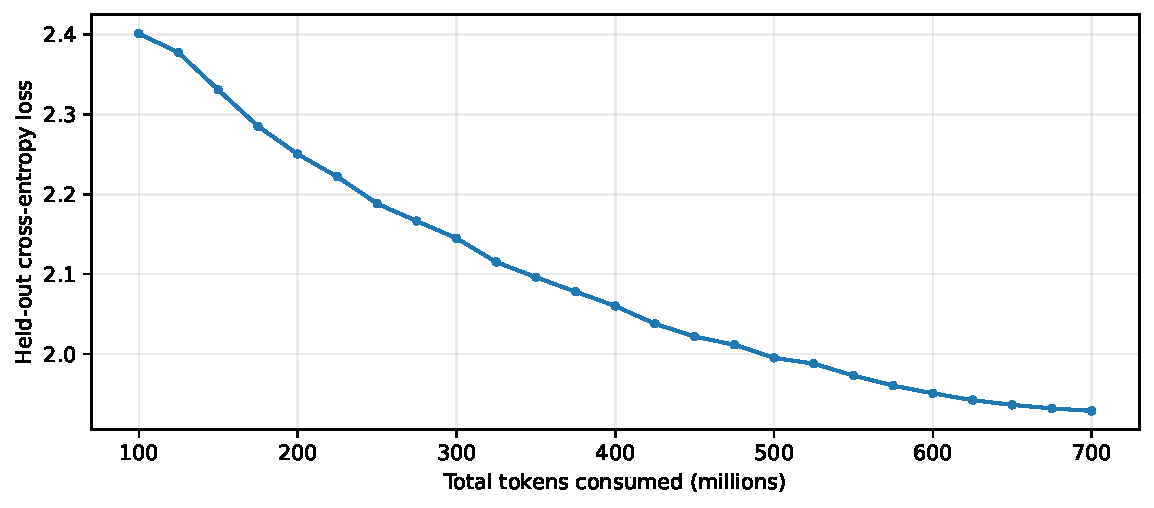
\includegraphics[width=.83\linewidth]{figures/phase1/p1_validation_curve.pdf}
\caption{Validation cross-entropy during continued Efficient-GQA pretraining, reconstructed from the actual notebook's displayed validation events. The initial 100M reference comes from the original architecture comparison and was measured in a different evaluation run; continuation observations follow the 25-batch schedule.}
\label{fig:valcurve}
\end{figure}

The trajectory in Figure~\ref{fig:valcurve} shows a generally monotonic decrease in held-out next-token loss, reaching approximately 1.9288 at 700M. This supports the narrow claim that the model became a better fit to its validation token distribution under the chosen cross-entropy objective. It does not establish a corresponding improvement in hidden-reference continuation overlap or legal factual correctness.

\subsection{Generation and decoding hypotheses}
For all official submissions the generated \method{text} field had to contain exactly 128 whitespace-separated words, excluding the original prompt. The initial submissions used temperature 0.8, top-\(k=50\), top-\(p=0.95\), repetition penalty 1.15, and a no-repeat four-token-gram guard. To avoid pathological outputs dominated by legal section numbers, dates or token sequences that rarely formed new words, the decoder reserved substantial context for generation and forced an alphabetic BPE token with leading whitespace after repeated non-word-start tokens. It seeded sampling deterministically from each prompt's SHA-1 digest, supported an emergency stronger guard for difficult cases, and truncated generated text only after reaching 128 words.

After reaching 500M, the experiment held model weights fixed and compared alternative decoding schedules on the pseudo-development set: conservative sampling, balanced sampling, low-temperature sampling, full-prompt greedy decoding, and the legacy guarded strategy. The decoder with the highest local ROUGE-L was selected for tuned submissions at 500M and 700M. Because this was a decoder-selection experiment and not an architecture experiment, the comparison is valid only for the local held-out continuation proxy; the private test result provides an additional generalization check.

\section{Results}
\subsection{Original architecture comparison}
The four independent submissions and the three continuation submissions were validly evaluated on the 1,000-example hidden-reference set. Table~\ref{tab:official} is the authoritative source of \emph{official} results for Phase 1. Values should not be mixed with local pseudo-development BLEU, which the notebook reports on a 0--100 scale.

\begin{table}[htbp]\centering\small
\caption{Official Codabench Phase-1 results, as transcribed from the seven user-provided score reports. The bold row is the winner according to the designated primary metric.}
\label{tab:official}
\begin{tabular}{lrrr}
\toprule Submission & BERTScore F1 & ROUGE-L F1 & BLEU-4 \\
\midrule
Decoder only, 100M & 0.83465570 & 0.19630469 & 0.05258763 \\
\textbf{Efficient GQA, 100M} & \textbf{0.83479506} & \textbf{0.19745313} & \textbf{0.05385350} \\
Efficient GQA, 300M & 0.83080482 & 0.17181250 & 0.03257670 \\
Efficient GQA, 500M tuned & 0.78932995 & 0.14202344 & 0.00777384 \\
Efficient GQA, 700M tuned & 0.80992270 & 0.14757031 & 0.01275489 \\
Encoder--decoder, 100M & 0.82569140 & 0.16444531 & 0.02212777 \\
Prefix-LM, 100M & 0.82551551 & 0.16594531 & 0.02618290 \\
\bottomrule
\end{tabular}
\end{table}

\begin{figure}[htbp]\centering
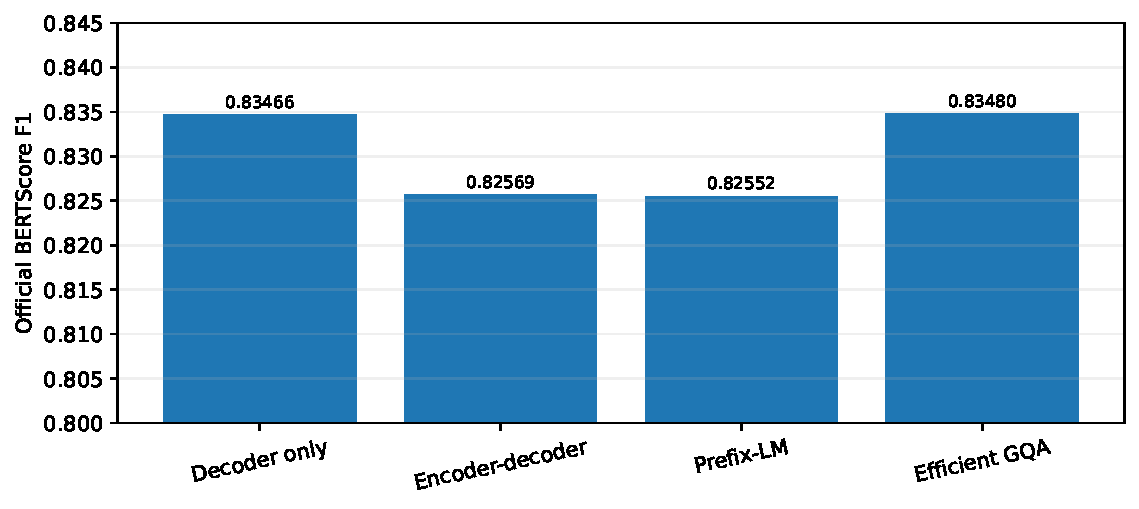
\includegraphics[width=.8\linewidth]{figures/phase1/p1_architecture_codabench.pdf}
\caption{Official primary scores of the original four 100M-token architectures. Efficient GQA wins narrowly over the standard decoder, while both beat encoder--decoder and prefix-LM.}
\label{fig:arch}
\end{figure}

The GQA model led the decoder-only model by approximately 0.00014 BERTScore F1. The architectures differ in several respects, and each score comes from one submission. The comparison therefore measures performance of the submitted systems without isolating the effect of grouped-query attention.

\subsection{Training-scale and private-test generalization gap}
\begin{figure}[htbp]\centering
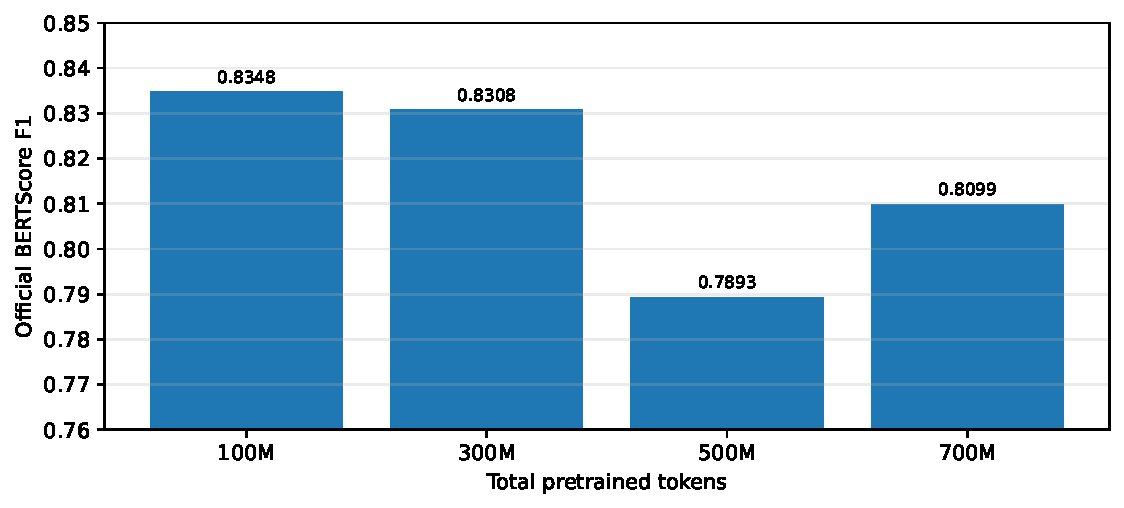
\includegraphics[width=.79\linewidth]{figures/phase1/p1_gqa_token_scaling.pdf}
\caption{Primary-score trajectory across the four Efficient-GQA submissions. Later checkpoints used an expanded training corpus; the 500M/700M submissions also used a different, locally tuned decoding configuration. This is not a controlled one-variable pretraining ablation across all points.}
\label{fig:scaling}
\end{figure}

The 700M validation loss fell to approximately 1.9288 (perplexity \(\approx6.88\)), whereas the original ~100M architecture-comparison perplexity was 11.039. Yet private BERTScore declined from 0.83479506 at 100M to 0.83080482 at 300M, 0.78932995 at 500M tuned, and 0.80992270 at 700M tuned. The largest official drop coincides with both continued training and an altered decoder; therefore this experiment cannot causally attribute the entire decline to more training tokens. It does, however, unequivocally reject the simple selection rule ``lower validation perplexity implies higher private-test BERTScore.''

\subsection{Decoding ablation and local-test discrepancy}
\begin{table}[htbp]\centering\small
\caption{500M checkpoint decoder screening on 40 balanced pseudo-development examples. Local BLEU-4 is reported in sacrebleu's 0--100 scale.}
\label{tab:decoding}
\begin{tabular}{lrr}
\toprule Decoder & Mean ROUGE-L F1 & BLEU-4 (0--100) \\
\midrule
Greedy full-prompt & \textbf{0.2837} & \textbf{15.7469} \\
Low-temperature sampling & 0.2737 & 15.0160 \\
Conservative sampling & 0.2634 & 14.3891 \\
Balanced sampling & 0.2546 & 13.2641 \\
Legacy word guard & 0.2313 & 10.7376 \\
\bottomrule
\end{tabular}
\end{table}

\begin{figure}[htbp]\centering
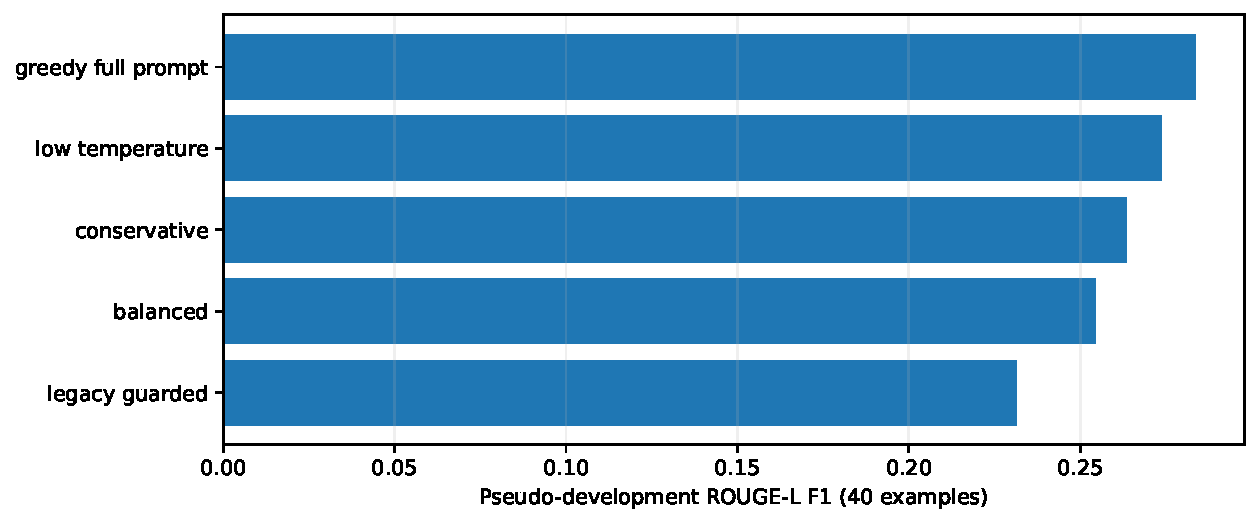
\includegraphics[width=.87\linewidth]{figures/phase1/p1_decoding_sweep.pdf}
\caption{The quick decoder ablation selected full-prompt greedy decoding on local overlap, but the official private-test metric favored the earlier 100M submission.}
\label{fig:decoding}
\end{figure}

The two best configurations were then reevaluated on all 160 pseudo-development examples. Greedy full-prompt obtained ROUGE-L F1 0.2933 and BLEU-4 18.8591, compared with 0.2761 and 16.5282 for low-temperature sampling. A separate 160-example evaluation of the 500M checkpoint with the original guarded decoder recorded 0.221375 and 10.102891. The 700M model using the selected greedy decoder achieved local ROUGE-L F1 0.2923 and BLEU-4 18.7765. The corresponding 500M and 700M official BERTScores were 0.78932995 and 0.80992270, both below the 100M winner. The local proxy and official metric have different targets. Comparing all checkpoints with the original decoder on the same official distribution would isolate the effect of the decoding change from other differences between submissions.

\subsection{Best official Phase-1 system}
The selected Phase-1 foundation for course submission is the \textbf{original approximately 100M-token Efficient-GQA best-validation checkpoint}, preserved as \method{milestones/best\_100M.pt} before subsequent training and used with the original \method{legacy\_word\_guard\_v1} generation code. The 300M, 500M, and 700M checkpoints are retained as completed experiments, not substituted for the winner. Only its winning inference path belongs in the final best-model-only code archive; all architecture and decoding experiments belong in the comprehensive GitHub research repository. The official competition rank was not present in the supplied score screenshots, so no numeric rank is asserted in this research edition.

\section{Error Analysis and Discussion}
\subsection{Observed failure modes during development}
The notebook's development logs document two concrete engineering problems. First, a rotary-embedding helper named \method{apply} conflicted with PyTorch's \method{nn.Module.apply}, causing model construction to fail when a recursive weight-initialization routine invoked it without the expected key/value arguments. Renaming the RoPE operation resolved the namespace collision. Second, early decoding generated many BPE tokens without enough whitespace-delimited words, especially numeral-heavy legal citation sequences. The initial rigid 128-word requirement then caused failed predictions despite exhausting the generation budget. This motivated the word-progress guard and conditional emergency retry used in valid submissions.

\subsection{Interpretation of the continuation results}
The full-corpus model improved at language modeling but not at the hidden continuation task. There are several plausible explanations, none established independently here: (i) the training data mixture shifted between the original cache and complete corpus; (ii) greedy decoding overoptimized the local proxy and reduced diversity or distributional overlap on official prompts; (iii) local pseudo-development continuations differ from the official hidden references; and (iv) a fixed 128-word target creates a length-control constraint not directly optimized by next-token cross entropy. Because multiple factors changed, a causal decomposition requires further controlled experiments. This is an important limitation of the experimental evidence, not a reason to discard negative results.

\paragraph{Evaluation limitations.} BERTScore rewards contextual semantic similarity to hidden reference continuations, ROUGE-L measures longest-common-subsequence overlap, and BLEU measures weighted clipped n-gram precision. None by itself establishes whether a generated judgment is factually accurate, cites a real statute, avoids fabricated case law, preserves privilege, or is suitable for legal decision-making. There was no reported expert legal assessment, no calibrated uncertainty for legal facts, and no verification against an external authority (the latter was disallowed by the official training-data restrictions).

\paragraph{Reproducibility.} The training notebook contains cells that restore runtime state after disconnections. The repository uses explicit configuration and automatic checkpoint loading. Exact replay still requires strict loading of the original weights and comparison of fixed-prompt logits and predictions with the archived run. The official Codabench scores come from the recorded submissions. Local evaluation uses the pseudo-development references.

\section{Conclusion and Next Steps}
Phase 1 delivered a from-scratch, legal-domain, self-hostable language foundation within the competition's parameter limit. Four different Transformer architectures were implemented and submitted, and the original 112.679M-parameter GQA model obtained the strongest private BERTScore (0.83479506). The experiments subsequently expanded the available training corpus to 4.488B BPE tokens and continued the same model to 700M consumed tokens. A declining next-token validation loss was not a reliable proxy for the private continuation metric, and a decoding rule that improved local ROUGE substantially did not transfer to official evaluation. The outcome supports a conservative model-selection procedure that prioritizes held-out task performance over optimization-loss improvements and documents configuration changes precisely.

The next research steps are to (a) compare checkpoints under an unchanged decoder and matched local evaluation set, (b) quantify source-dependent error rates using a fixed analysis subset, (c) inspect citation hallucination and repetition with a human-readable audit, and (d) transfer the chosen 100M foundation to later legal NLP tasks with explicit ablations of frozen, partial, adapter-based, and full fine-tuning. No privileged client data were used in this study; deployment suitability still requires security validation and human legal review.

\clearpage
\section{Phase 2: Legal Named Entity Recognition}
\label{sec:phase2}
The second phase adapts the Phase 1 legal models to extract typed entities from full judgments. The official output is one list of \([s,e,\ell]\) triples per document ID, with zero-based character offsets, an exclusive end, and a label from the twelve official types. Strict evaluation matches both boundaries and the label. The primary metric averages class-wise \(F_1\) equally across the twelve classes. Micro-\(F_1\) pools exact true positives, false positives, and false negatives before scoring. Codabench evaluates 35 judgments from fold 3 using private gold labels.

\subsection{Data, split, and character alignment}
Folds 1 and 2 provide 35 labeled judgments each, with 8,393 annotated entities. The median judgment is 26,620 characters and the longest is 114,044. All 70 exceed 1,280 BPE tokens in the archived tokenization analysis. Figure~\ref{fig:p2-support} shows the annotation imbalance. DATE has 1,575 instances, compared with 184 for R.COUNSEL. The original protocol sampled 3,000 document partitions, each holding out seven judgments from each fold, and minimized the mean deviation from a 20\% per-class holdout with a penalty for missing classes. The selected partition has 56 training judgments with 6,667 annotations and 14 validation judgments with 1,726 annotations. Both contain all classes. The final retraining uses all 70 labeled judgments and retains the fixed test fold.

\begin{figure}[htbp]\centering
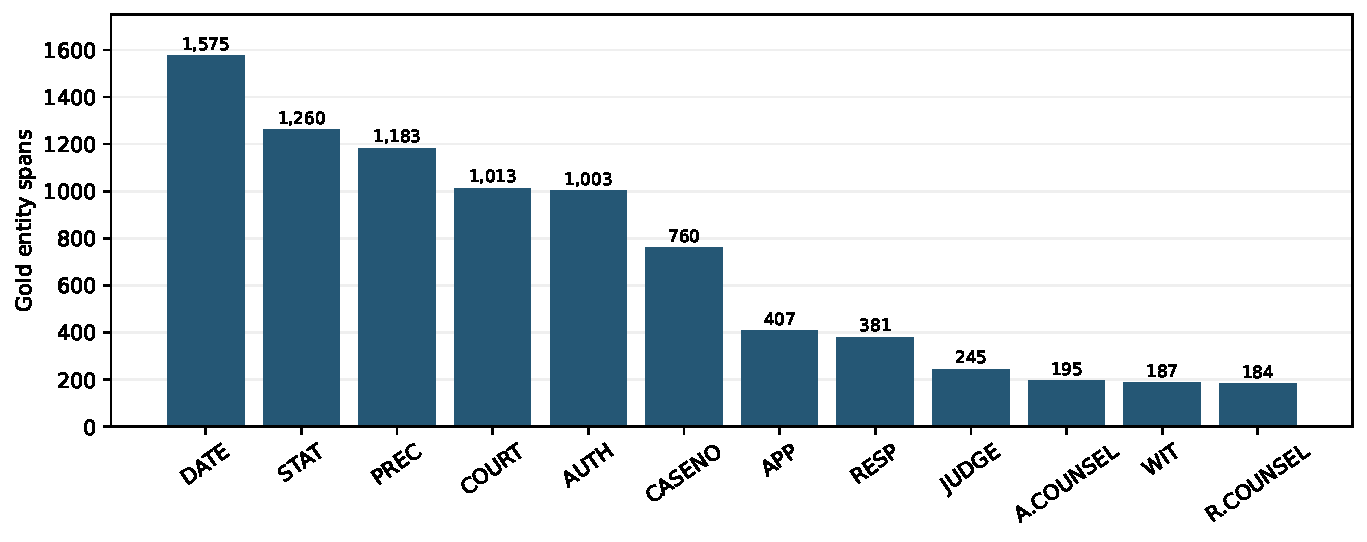
\includegraphics[width=.88\linewidth]{figures/phase2/p2_class_support.pdf}
\caption{Entity support across the 70 labeled judgments. Strict macro-\(F_1\) gives each of these classes equal weight.}
\label{fig:p2-support}
\end{figure}

The supplied gold mention strings agreed with every end-exclusive slice. We preserve the document characters and use the archived legal byte-level BPE tokenizer. Trimming whitespace from token offset intervals raised exact boundary alignment from 3.66\% to 98.19\%. A span receives a beginning tag and inside tags only if its endpoints coincide with usable token boundaries. Unrepresentable spans mask overlapping tokens during training. Whitespace-only tokens are also ignored. Decoding gold BIO tags reconstructed 8,241 spans with zero false positives and strict macro-\(F_1\) of 0.99319 on the labeled documents. This oracle quantifies representation loss on those judgments. It uses the gold tags.

Each training or inference window owns up to 256 tokens and carries up to 128 tokens of context on either side. Only owned tokens contribute to the BIO loss. There are 1,491 training, 342 validation, and 976 test windows. The full-data training set contains 1,833 windows. At inference, the system reassembles the owned token predictions in document order before converting BIO tags to character spans. A beginning tag starts a span, as does an inside tag with no active span of its type. Reassembly allows entities to cross an ownership boundary.

\subsection{Adaptation and training protocol}
All systems use a 25-way BIO classification head with dropout 0.1. The full GQA and decoder systems retain causal attention. The two adapter families use bidirectional attention on each window and mask padded keys.

\begin{itemize}[leftmargin=*]
\item \textbf{Frozen probe.} The 100M-token Efficient GQA foundation is fixed. The 19,225-parameter head learns for four epochs at \(2\times 10^{-3}\), with entity-tag weight 2 and outside-tag weight 1.
\item \textbf{Full fine-tuning.} The GQA foundation uses the archived best-through-700M-token snapshot, and the decoder uses its 100M-token snapshot. Each model updates the backbone at \(2\times 10^{-5}\) and the head at \(3\times 10^{-4}\), using plain token cross-entropy and up to four epochs.
\item \textbf{Encoder LoRA.} The 100M-token encoder--decoder contributes its encoder states. Rank-16 additive adapters with scaling \(32/16\) and dropout 0.05 target the encoder attention input and output projections. The frozen base and the trainable BIO head give 446,105 trainable parameters in total. The first run uses plain cross-entropy. The balanced run uses the same adapter initialization and batch schedule, outside-tag weight 0.2, and entity-tag weight 1.
\item \textbf{Prefix-LM LoRMA+.} On the 100M-token Prefix-LM, the notebook's rank-16 residual multiplicative adapter computes \(z=W_0x\) and \(z+(32/16)BAz+b\) on each attention projection. The base weights are frozen and their dropout is disabled. The adapter and head have 1,198,873 trainable parameters. The outside-tag weight is 0.5. The implementation uses the LoRA and LoRMA families described by \href{https://arxiv.org/abs/2106.09685}{Hu et al.} and \href{https://aclanthology.org/2025.findings-acl.527/}{Mao et al.}, with the projection and bias conventions of the executed notebook.
\item \textbf{Seven-layer GQA students.} Both students start with embeddings, final normalization, and blocks \(0,2,\ldots,12\) from Phase 1 GQA, and the same seeded new BIO head. The control uses plain cross-entropy. The distilled model minimizes \(0.7\,\mathrm{CE}+0.3\,T^2\,\mathrm{KL}(p_T\|q_T)\) on supervised tokens, with \(T=2\). Here \(p_T\) and \(q_T\) are temperature-scaled teacher and student distributions. The fine-tuned GQA teacher supplies cached per-window logits. Both student runs last four epochs.
\end{itemize}

Training uses AdamW with weight decay 0.01 and gradient clipping at norm 1. The full, adapter, and student runs accumulate gradients over 16 windows per update, using a 6\% warmup and linear decay. The adapter/head learning rates are \(3\times 10^{-4}\) and \(8\times 10^{-4}\). The student backbone/head rates are \(3\times 10^{-5}\) and \(3\times 10^{-4}\). The adapter budget is six epochs, with early stopping on strict validation macro-\(F_1\). The original trained models are selected by that same validation metric. Full-data training uses four fixed epochs for GQA, decoder, and student, and takes their final weights. Its student uses the full-data GQA teacher.

\subsection{Exact-span voting and validation}
Full GQA, full decoder, and the distilled student each cast one vote per span. Majority voting accepts a span only when at least two members predict the same start, end, and label. Candidates are considered by decreasing vote count, GQA support, and span length, then by ascending span tuple. A candidate is skipped if it overlaps a span already accepted. The rule applies independently to each judgment.

\begin{table}[htbp]\centering\small
\caption{Five voting rules on the original 14 validation judgments.}
\label{tab:p2-votes}
\begin{tabular}{lrrrrr}
\toprule
Rule & Macro-\(F_1\) & Micro-\(F_1\) & TP & FP & FN \\
\midrule
Majority & \textbf{0.30658} & 0.45496 & 654 & 495 & 1,072 \\
GQA confirmed by another member & 0.30323 & \textbf{0.46406} & 623 & 336 & 1,103 \\
GQA or agreement of both other members & 0.27031 & 0.35830 & 696 & 1,463 & 1,030 \\
Union & 0.24391 & 0.30967 & 722 & 2,215 & 1,004 \\
Unanimous & 0.22975 & 0.44444 & 522 & 101 & 1,204 \\
\bottomrule
\end{tabular}
\end{table}

Majority voting led the strongest single model by 0.03982 macro-\(F_1\) and reduced false positives from 1,435 to 495. Same-label boundary errors fell from 828 to 260 and spurious spans from 381 to 140. The improvement involved a precision--recall trade-off. The ensemble dropped 26 true positives and increased false negatives from 1,046 to 1,072. For R.COUNSEL, \(F_1\) fell from 0.09259 to 0.02817. Before resolving overlaps, exact precision rose from 5.45\% for spans predicted by one member to 25.10\% for two and 83.79\% for three. The models' pairwise exact-span Jaccard scores ranged from 0.213 to 0.245.

Across 500 paired bootstrap resamples of the 14 validation documents, the archived mean ensemble gain was 0.04446 and the central 95\% range was [0.02328, 0.07227]. The same validation set selected the voting rule and supplied the bootstrap draws. This interval describes variation within that analysis and does not estimate an independently selected system's gain on unseen documents.

\subsection{Local and official results}
\begin{table}[htbp]\centering\small
\caption{Phase 2 model results. Validation scores use the selected epoch or voting rule. A dash indicates an unavailable score. The three individual full-data ZIPs were archived. Official scores are available for seven submissions.}
\label{tab:p2-results}
\begin{tabular}{lrrr}
\toprule
Model & Validation macro-\(F_1\) & Codabench macro-\(F_1\) & Submission ID \\
\midrule
GQA frozen probe & 0.16766 & -- & -- \\
GQA full & 0.26676 & 0.2960 & 971886 \\
Decoder full & 0.24495 & 0.2849 & 971879 \\
Encoder LoRA & 0.02086 & -- & -- \\
Encoder LoRA balanced & 0.04995 & 0.0459 & 971880 \\
Prefix-LM LoRMA+ & 0.06334 & 0.0651 & 971887 \\
Seven-layer GQA supervised & 0.24068 & -- & -- \\
Seven-layer GQA distilled & 0.25122 & 0.2736 & 971885 \\
Original majority ensemble & \textbf{0.30658} & 0.3342 & 971884 \\
Full-data GQA & -- & -- & -- \\
Full-data decoder & -- & -- & -- \\
Full-data distilled GQA & -- & -- & -- \\
Full-data majority ensemble & -- & \textbf{0.3577} & \textbf{971881} \\
\bottomrule
\end{tabular}
\end{table}

\begin{figure}[!htb]\centering
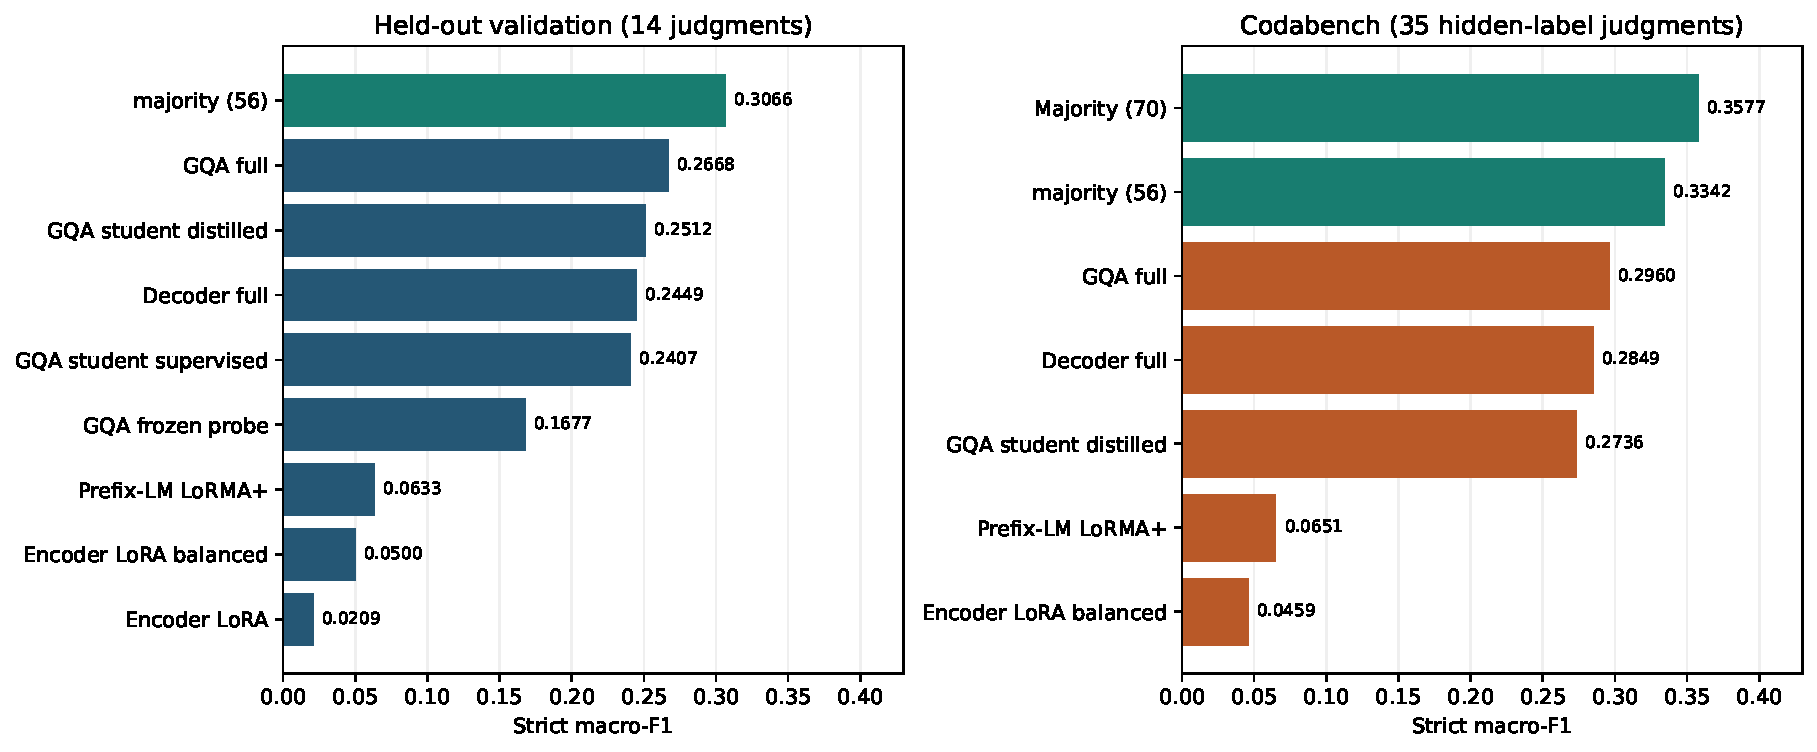
\includegraphics[width=\linewidth]{figures/phase2/p2_strict_results.pdf}
\caption{Local model selection and official Codabench scores on different sets of judgments. The full-data ensemble used all labeled documents and has no independent validation score.}
\label{fig:p2-results}
\end{figure}

Distillation raised the student's validation macro-\(F_1\) by 0.01054 against the equally sized supervised control. The student has 68.65M parameters versus the 112.70M-parameter teacher, a 39.1\% reduction, and scored 0.2736 on Codabench. The teacher scored 0.2960. The notebook's repeated evaluation of the frozen probe and the teacher in separate analysis cells yielded small differences from the selected validation scores. The registry keeps these measurements separate.

The strongest official project submission is the full-data majority ensemble, with strict macro-\(F_1\) of \textbf{0.3577} (ID 971881). Its 0.0235 gain over the original majority ensemble compares the two submitted systems. The retraining changed training coverage, seeds, and selection protocol, so the gain cannot be attributed to the additional judgments alone. The Codabench screenshot establishes the reported scores for these submissions. Hidden class-wise scores and overall competition rank are unavailable.

\subsection{Why the adapter scores may be weak}
\paragraph{Observed behavior.}
The outside tag accounts for 341,310 of 374,030 supervised training tokens (91.25\%). Original LoRA scored zero validation macro-\(F_1\) in its first two epochs while its training loss fell. All 14 LoRA \(B\) tensors had nonzero norms at the selected checkpoint, and a small training-document sample still scored just 0.04136 strict macro-\(F_1\). The balanced variant raised macro recall from 0.02898 to 0.10782 and validation macro-\(F_1\) from 0.02086 to 0.04995. False positives rose from 1,257 to 8,235 as true positives rose from 71 to 286. Prefix-LM LoRMA+ peaked at 0.06334 in epoch 3 while training loss continued to fall. It produced 246 true positives and 4,646 false positives on validation, with zero exact hits for RESP, A.COUNSEL, and WIT.

\begin{figure}[!htb]\centering
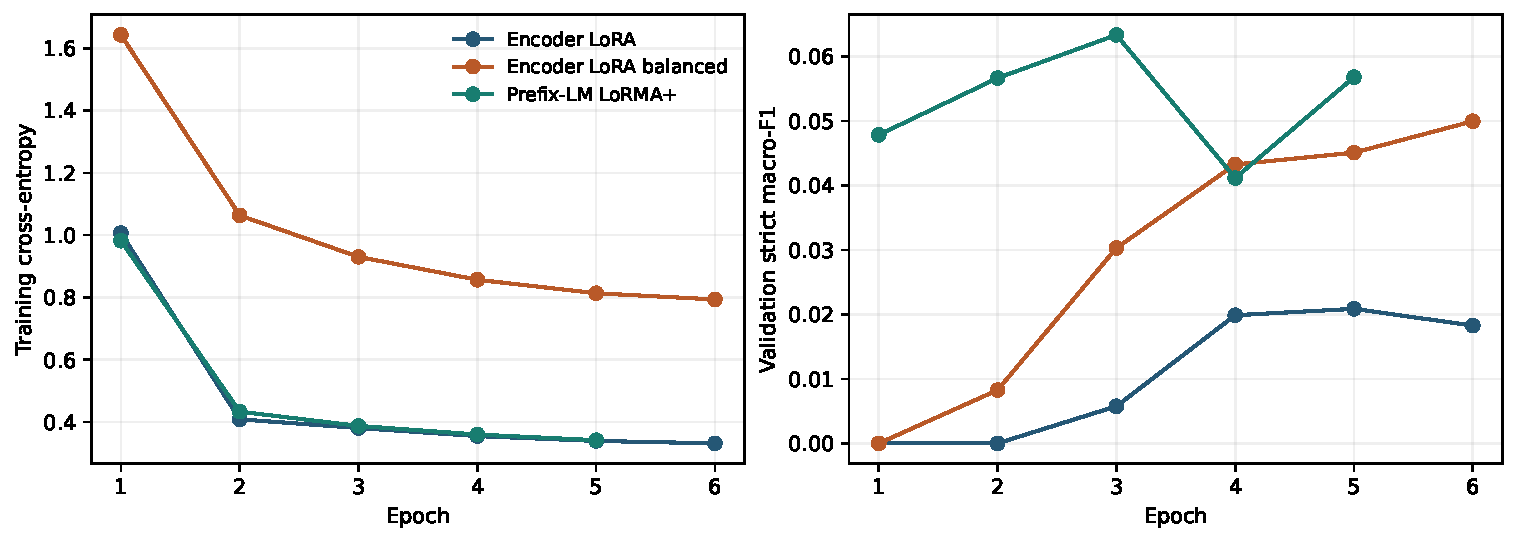
\includegraphics[width=.95\linewidth]{figures/phase2/p2_adapter_training.pdf}
\caption{Executed adapter training histories. Cross-entropy is comparable across epochs within each run. The runs use different outside-tag weights.}
\label{fig:p2-adapters}
\end{figure}

\paragraph{Plausible explanations.}
Plain token cross-entropy gives the frequent outside tag most of the supervised positions. Reducing its weight may improve sensitivity while encouraging extra entities, as observed for balanced LoRA. Token-level loss also gives partial credit to correctly tagged tokens inside a span, whereas strict scoring requires both endpoints and the class. The high BIO oracle score suggests alignment loss alone is too small to explain the measured adapter scores on labeled data. Limited rank, adapting only attention projections, and reusing frozen features from a language-modeling objective may each restrict transfer to boundary detection and role typing. The small number of annotated documents, uneven class support, and the 512-token context may also limit evidence for rare roles and long-range references.

\paragraph{Limits of attribution.}
The adapters used different architectures, pretraining snapshots, attention behavior, class weights, and trainable fractions from the fully fine-tuned models. The study contains one validation partition and one execution per main configuration. It does not isolate rank, projection targets, foundation quality, or calibration effects. The balanced LoRA comparison supports a sensitivity trade-off in this setting. The weaker adapter scores establish the outcome of these configurations on this task, with matched-backbone and repeated-seed comparisons needed to separate the possible mechanisms.

\subsection{Reconstruction checks}
The released pipeline regenerated the archived split and all 105 token records from the official files and tokenizer. All twelve archived submissions passed document ID, label, offset, and ZIP structure checks. Both ensemble submissions were reproduced span for span from their archived members, and the five validation voting scores and paired diagnostics were reproduced from the saved validation predictions. The probe head and three adapter states loaded into the reconstructed models. Large original backbones and full-model checkpoints exceeded the available Drive transfer limit, leaving original-weight inference and training replay unverified. The recorded Codabench scores come from the submitted archives and the supplied score screenshot.


% Phase 3: archived numerical results, original executed notebook, and official Codabench screenshot.
% Reproduce figures from code/phase3/analysis/figures.py; do not edit scores by hand.
\clearpage
\section{Phase 3: Sentence-Level Rhetorical Role Prediction}
\label{sec:phase3}

\subsection{Research question and task formulation}
Legal decisions contain factual narratives, petitions, statutory references, earlier decisions, reasoning and operative rulings. The same sentence may communicate evidence, an advocate's position, or a court's conclusion depending on surrounding sentences. We therefore cast rhetorical-role prediction as contextual sentence classification while preserving the order of an entire judgment. For a judgment $D=(s_1,\ldots,s_n)$ with a target sentence $s_i$ and optionally its neighboring context $C_i$, the classifier produces
\begin{equation}\label{eq:p3-task}
 p_\theta(y_i=k\mid s_i,C_i)=\operatorname{softmax}(\mathbf W h_\theta(s_i,C_i)+\mathbf b)_k,\qquad
 \hat y_i=\arg\max_{k\in\{1,\ldots,13\}}p_\theta(y_i=k\mid s_i,C_i).
\end{equation}
\begin{sloppypar}
The official label vocabulary is exactly \method{Fact}, \method{Issue}, \method{Argument\allowbreak Petitioner}, \method{Argument\allowbreak Respondent}, \method{Statute}, \method{Dissent}, \method{Precedent\allowbreak Relied\allowbreak Upon}, \method{Precedent\allowbreak Not\allowbreak Relied\allowbreak Upon}, \method{Precedent\allowbreak Overruled}, \method{Ruling\allowbreak By\allowbreak Lower\allowbreak Court}, \method{Ratio\allowbreak Of\allowbreak The\allowbreak Decision}, \method{Ruling\allowbreak By\allowbreak Present\allowbreak Court} and \method{None}. The label-to-index mapping is read directly from the supplied \path{label_vocab.json}; names and capitalizations are not rewritten. Every prediction list must have the same length as the original document's sentence list.
\end{sloppypar}

The official primary metric is macro-averaged F1 over \emph{all} 13 roles, including roles with zero development support:
\begin{equation}\label{eq:p3-f1}
\mathrm{MacroF1}=\frac1{13}\sum_{k=1}^{13}\frac{2\,\mathrm{TP}_k}{2\,\mathrm{TP}_k+\mathrm{FP}_k+\mathrm{FN}_k},\qquad 0/0:=0.
\end{equation}
Macro-precision and macro-recall are companion measures. A low-frequency label may have a large effect on Macro-F1 despite contributing few sentences. The experiment set therefore investigated four original Phase-1 architectures, multiple adaptation mechanisms, sentence context, domain-specific learning, structured label decoding, class balancing and knowledge distillation.

\subsection{Dataset and evidence integrity}
\label{sec:p3-data}
All data originate from \method{Exploration-Lab/CS-781-Capstone}, folder \method{Phase\_3\_RR}; no external pretrained language models or training corpora were used. The train/development lists each comprise document records with \method{id}, an ordered \method{text} sentence array and aligned \method{labels}; hidden-test files instead map document IDs directly to sentence arrays. This structural distinction was discovered during ingestion and handled explicitly, without changing sentence order.

\begin{table}[htbp]\centering\small
\caption{Exact Phase-3 data sizes from the completed exploratory notebook. Train/dev include labels; test labels are withheld.}
\label{tab:p3-sizes}
\begin{tabular}{@{}lrrr rrr@{}}\toprule
 & \multicolumn{3}{c}{Documents} & \multicolumn{3}{c}{Sentences}\\
Domain & Train & Dev & Test & Train & Dev & Test\\\midrule
Corporate Law (CL) & 40 & 5 & 5 & 10,593 & 1,396 & 1,339\\
Information Technology (IT) & 40 & 5 & 5 & 6,252 & 746 & 858\\
\midrule
Total & 80 & 10 & 10 & 16,845 & 2,142 & 2,197\\\bottomrule
\end{tabular}
\end{table}
The mean sentence count alone is misleading because judgments vary considerably in length: the largest training document has 1,816 sentences in CL and 442 in IT, whereas the median counts are 120.5 and 126.5 respectively. Document-level leakage matters: the notebook checked 100 documents across train/dev/test and found no exact normalized-text duplicate across different splits, no overlapping domain IDs and no blank sentences. These are \emph{exact-match} integrity checks, not exhaustive near-duplicate detection.

\begin{figure}[htbp]\centering
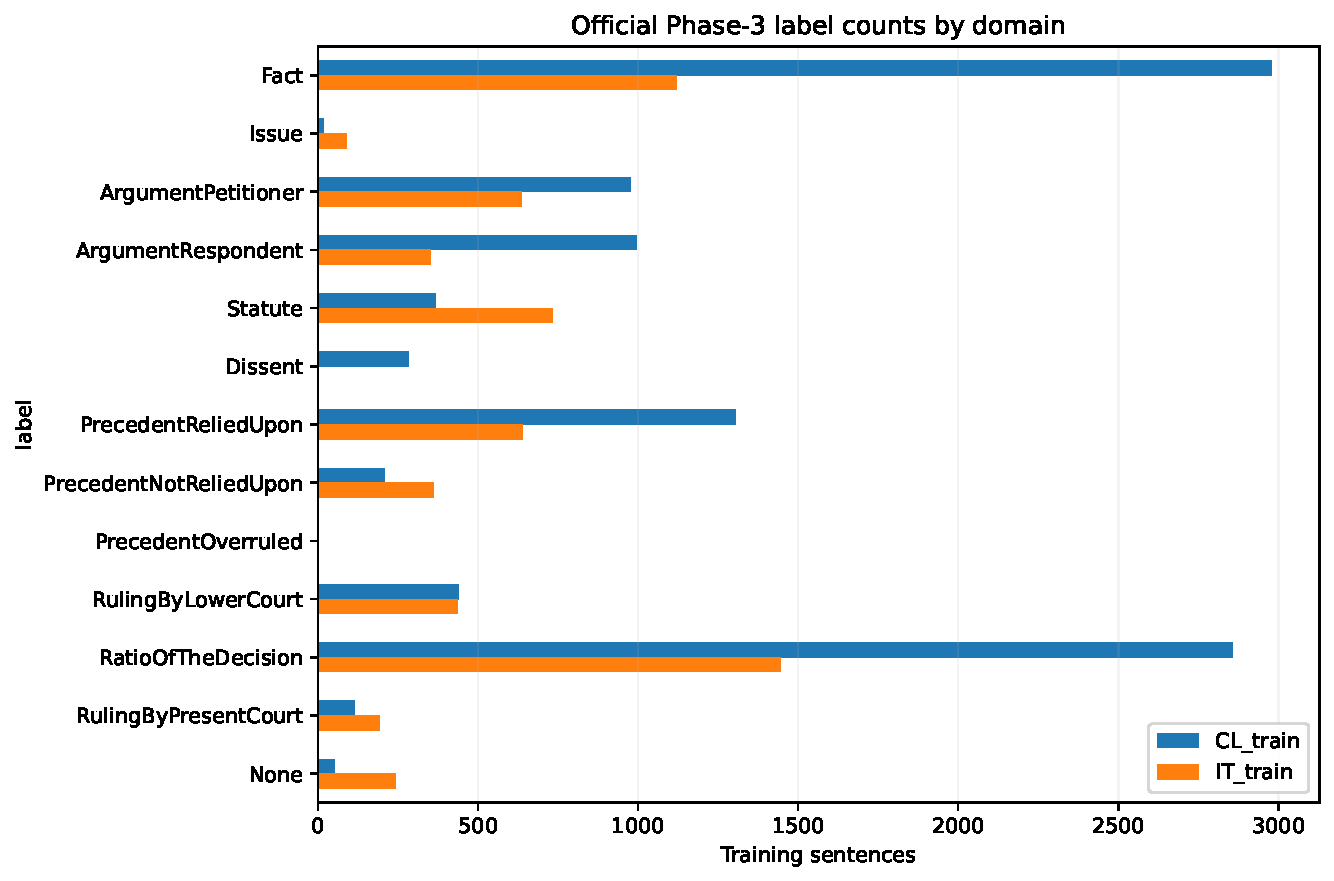
\includegraphics[width=.86\linewidth]{figures/phase3/p3_label_distribution.pdf}
\caption{Training-role distribution by legal domain, based on the official label counts recorded in the notebook. Both domains are imbalanced and differ substantially in the use of certain roles.}
\label{fig:p3-labels}
\end{figure}
\method{Fact} appears 2,979 times in CL training but 1,119 times in IT; \method{Ratio\allowbreak Of\allowbreak The\allowbreak Decision} appears 2,856 and 1,445 times. The rare \method{Precedent\allowbreak Overruled} occurs only three times in IT training and zero times in CL; \method{Dissent} occurs 284 times in CL training and zero times in IT. \method{Issue} appears 17 times in CL and 90 times in IT. Consequently, class weighting cannot solve all low-support errors: in particular, no method can infer an absent class from same-domain supervised examples alone. There are 0 examples of both \method{Dissent} and \method{Precedent\allowbreak Overruled} in the 2,142-sentence development set, so their reported per-class F1 scores are zero by the explicit 13-label convention.

\subsection{Tokenization, sentence representation and truncation}
\label{sec:p3-preprocess}
The original Phase-1 legal byte-level BPE tokenizer was recovered as \path{legal_bpe_32k.json} (32,000 entries; pad, BOS, EOS and UNK IDs $0,1,2,3$). No new BPE was fit for this phase. Sentences were tokenized without automatic specials, then packed as BOS + content + EOS. The pooled training-token distribution had its 95th percentile below 128, so the notebook fixed its maximum input length to 128 BPE tokens. The observed fraction of single-sentence training inputs beyond 128 tokens was 1.38\% for CL and 2.85\% for IT. Overlong sentences were shortened by keeping 75\% of the available budget from the beginning and 25\% from the end. This preserves some late conclusions but can remove legally salient clauses in the middle; it is an explicit information-loss limitation.

For the causal decoders, the 768-dimensional hidden representation at the \emph{last non-padding EOS position} is used for classification. Causal masking makes right padding invisible to that location. The Prefix-LM variant was run with full-sentence bidirectional attention and an explicit key-padding mask. The encoder--decoder variant used only the pretrained encoder, with its own padding-safe attention, not the pretrained cross-attentive decoder. These architectural distinctions matter: transferring the encoder only is not a direct measure of the usefulness of the model's pretrained decoder or the original sequence-to-sequence generation objective. The 13-class head is a dropout layer followed by a linear projection.

\begin{figure}[htbp]\centering
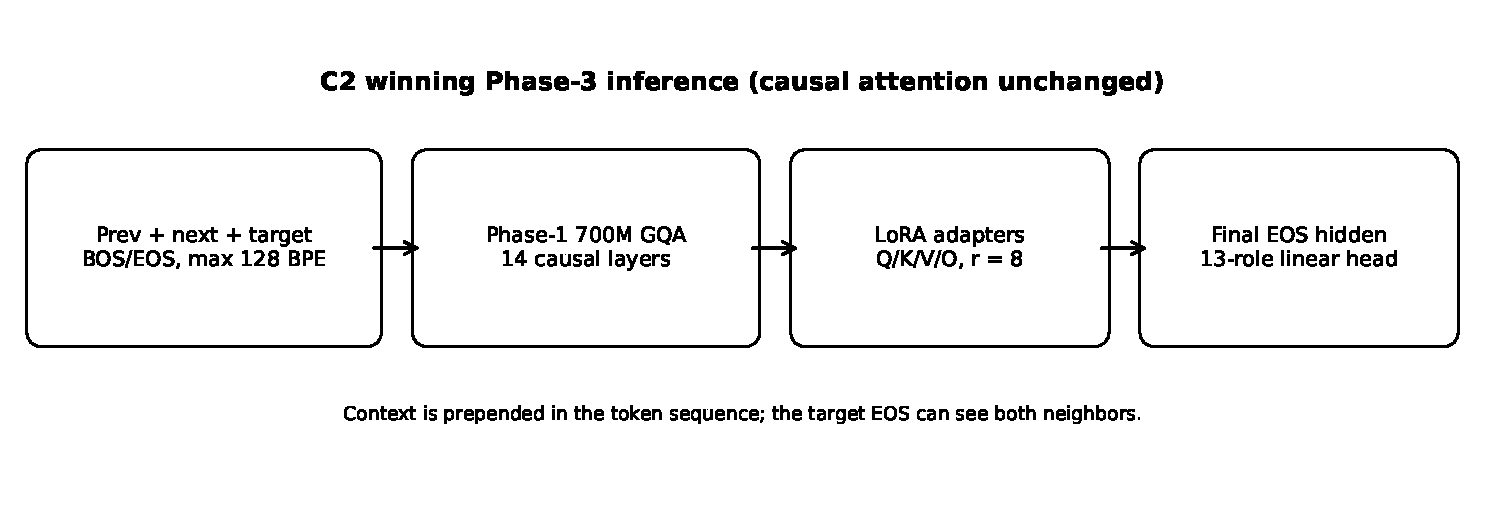
\includegraphics[width=.96\linewidth]{figures/phase3/p3_c2_architecture.pdf}
\caption{Actual C2 winning pipeline. Neighboring sentences are placed before the target under an unchanged causal 14-block Efficient GQA backbone; rank-8 LoRA adapters modify attention projections, and the final target EOS hidden state feeds a 13-class head. This is a schematic of executed inference, not a separately trained document encoder.}
\label{fig:p3-c2-architecture}
\end{figure}

\subsection{Adaptation methods and supervised optimization}
\label{sec:p3-methods}
The 14-block Phase-1 Efficient GQA model (768 hidden, 12 query heads, four KV heads, RoPE, RMSNorm and SwiGLU) was the principal backbone. Phase 3 used both the preserved 100M-token milestone and the continuation to approximately 700M consumed pretraining tokens. The four-architecture screening additionally used the original decoder-only, encoder--decoder and Prefix-LM backbones.

For frozen-base \emph{LoRA}, each selected attention projection received an additive rank-$r$ update,
\begin{equation}\label{eq:p3-lora}
 W' x=W_0 x+\frac{\alpha}{r}BAx,
\end{equation}
with $r=8$, $\alpha=16$ and adapter dropout 0.05. \emph{LoRMA+} used a different, multiplicative \emph{output-side} transformation of a base projection,
\begin{equation}\label{eq:p3-lorma}
 W' x=\left(I+\frac{\alpha}{r}BA\right)W_0x,
\end{equation}
initialized to the identity by setting $B=0$. All GQA attention projection biases are absent in the original architecture. \emph{IA$^3$} learned output scaling vectors for key/value projections and input scaling for the SwiGLU down projection; it did not update full projection matrices. \emph{Prefix tuning} learned 16 virtual key/value vectors per attention layer, visible to every real token while retaining causal real-token attention. The full-fine-tuning comparison updated all pretrained GQA parameters and the head. These were genuine changes of adaptation mechanism, not rank or learning-rate sweeps.

All main configurations used three-epoch budgets, AdamW with weight decay 0.01, batch size eight, two microbatches per optimizer update, gradient clipping to 1, a 5\% warmup followed by cosine decay, and development Macro-F1 checkpoint selection. Frozen-backbone adapter runs used learning rate $1.5\times10^{-4}$; full and student fine-tuning used $3\times10^{-5}$. Where supported, inference and training used BF16 autocasting. Model/head checkpoints and resumable optimizer states were saved separately in Drive; most training variants used a checkpoint every 300 optimizer updates, and the architecture-screening stage saved every 250 training batches. The best saved epoch was selected on development Macro-F1 and used for test inference. The original notebook contains one run per main condition, not repeated-seed estimates; dev-set tuning risks optimism with just ten judgments.

\subsection{Study design and actual experiment chronology}
\label{sec:p3-experiment-design}
\paragraph{Group A: four pretrained architectures and continued pretraining.}
A1--A4 held the LoRA method fixed while comparing standard causal decoder, encoder--decoder encoder, Prefix-LM and Efficient GQA (100M). A5 replaced only A4's foundation snapshot with the 700M GQA milestone. On development Macro-F1, the original GQA scored 0.3073 and the continued GQA 0.3291. The latter is a transfer improvement in this same-backbone comparison; the four-way architectural comparison still involves different objectives, dimensions, pooling and parameter counts.

\paragraph{Group B: adaptation mechanisms.}
On the 700M GQA, additive LoRA reached 0.3291 development F1; LoRMA+ reached 0.3171, IA$^3$ 0.2288, virtual prefix tuning 0.1983 and full fine-tuning 0.3330. Trainable parameter counts were respectively 583,437, 468,749, 45,837, 124,685 and 112,688,653. The full-fine-tuning gain over LoRA was only 0.0038 locally under these settings; without repeated seeds the experiment does not establish practical parity between the methods. The LoRMA+ official submission showed \method{Failed}, and the IA$^3$ submission showed \method{Preparing} in the supplied Codabench screenshot; both remain completed local training experiments and valid local prediction archives, but are not confirmed official evaluations.

\paragraph{Group C: context and structured decoding.}
C1 constructed \method{[BOS] [previous] [EOS] [target] [EOS]}. C2 constructed {\ttfamily\small [BOS] [previous] [EOS] [next] [EOS] [target] [EOS]}, omitting nonexistent neighbors at document boundaries. Context was budgeted inside the same 128-token limit; the target received at most about 65\% of the 126 content tokens, with remaining tokens divided between neighbors. Importantly, this is \emph{not} a bidirectional self-attention model: the GQA transformer remains causal, but the EOS summary of the final target can attend to tokens from both neighbors because both neighbors are placed earlier in the packed input. This design directly investigates the impact of legal discourse context.

C1 improved pooled dev Macro-F1 to 0.3424 and C2 to \textbf{0.3851}, versus 0.3291 without context. C3 instead estimated smoothed start-label and label-transition probabilities from training documents and performed document-wide Viterbi decoding on A5 emission log-probabilities. Transition strengths $\{0,.15,.30,.50,1,1.5,2\}$ were scored on development labels; 0.30 achieved 0.3527. This is a document-level \emph{structured postprocessor}, not a full-document neural text encoder or CRF-trained end-to-end. There was no hierarchical BiGRU, CRF or whole-judgment neural Transformer in the executed Phase-3 notebook.

\paragraph{Group D: joint versus domain-specific learning.}
D1 trained only CL judgments and D2 trained only IT judgments, evaluating each on both development domains. D1 achieved pooled 0.2215; D2 0.3020. Both lagged the joint A5 baseline (0.3291), although training-set sizes differed, so data volume and specialization are confounded. D3 used CL specialist outputs on CL test cases and IT specialist outputs on IT cases. This inference-only hybrid scored 0.3957 on the official hidden test, but the notebook did not record an independent development Macro-F1 for this hybrid; none is inferred here.

\paragraph{Group E: mandatory teacher--student knowledge distillation.}
The teacher was selected by development F1 among A5 and Group B, resulting in the fully fine-tuned GQA B4 at 0.3330. Both smaller students retained six layers $\{0,2,4,6,8,11\}$ from the original Phase-1 pretrained 12-layer decoder-only architecture, with 68,097,805 total parameters. E1 was trained using only hard labels. E2 used both ground truth and cached teacher-logit distributions:
\begin{equation}\label{eq:p3-kd}
 \mathcal L_{\rm KD}=\tfrac12\mathcal L_{\rm CE}+\tfrac12\, T^2 D_{\rm KL}\left(p_{\rm teacher}^{(T)}\Vert p_{\rm student}^{(T)}\right),\qquad T=2.
\end{equation}
E1 reached 0.3234 and E2 reached 0.3200 on development; corresponding official Macro-F1 scores were 0.3679 and 0.3638. Distillation therefore \emph{did not improve} predictive F1 in this controlled student comparison, although the smaller distilled student achieved about 3.69 times the teacher's measured sentence throughput (3,823 versus 1,035 sentences/s on the same fixed test subset). That benchmark measured throughput but did not isolate GPU memory: both models were resident simultaneously, so the reported peak GPU values are not reliable evidence of model-by-model peak-memory savings.

\paragraph{Group F: class-weighted loss.}
F1 used inverse-square-root class weights computed strictly from the training labels and clipped to $[0.2,5.0]$. It improved development Macro-F1 from A5's 0.3291 to 0.3459. Codabench displayed a numeric 0.3703 but also the \method{Failed} status; this cannot be counted as a confirmed official result without the failure details. It is nonetheless a meaningful local experiment.

\begin{figure}[htbp]\centering
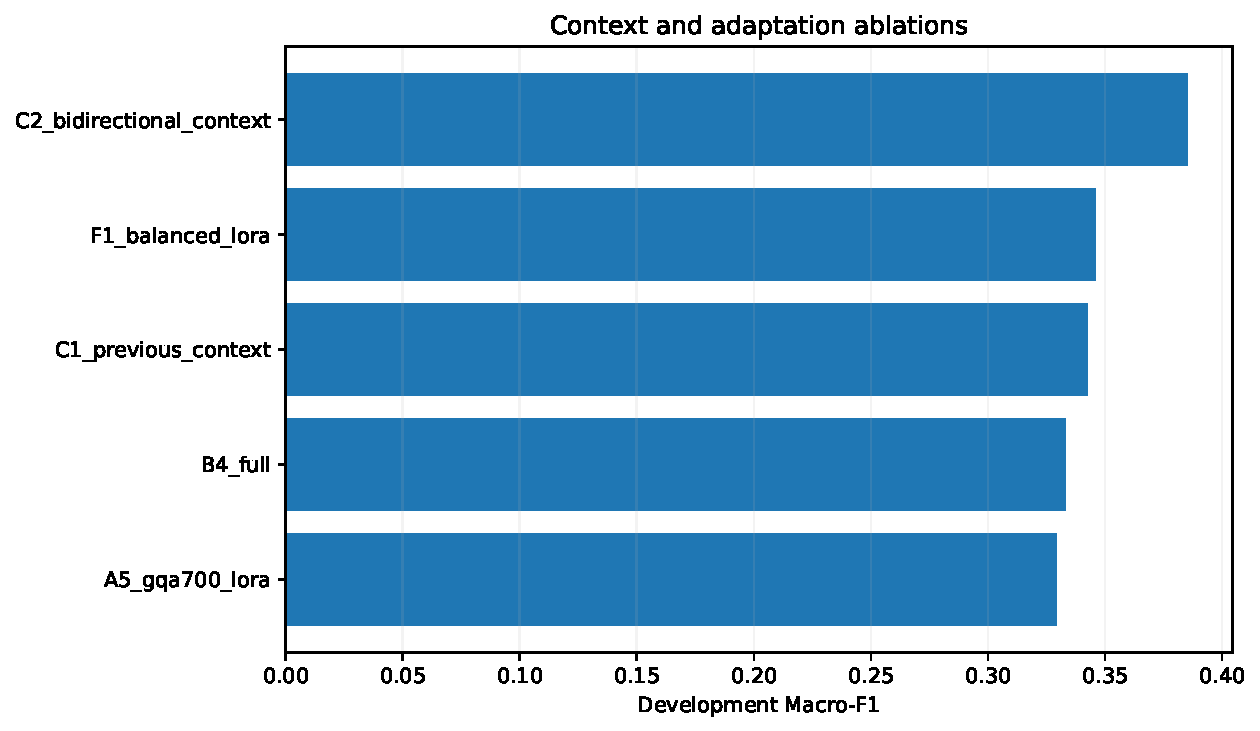
\includegraphics[width=.86\linewidth]{figures/phase3/p3_context_ablation.pdf}
\caption{Selected single-run development Macro-F1 results. The gain from C2 is measured against a shared 700M-GQA LoRA baseline with the same 128-token input budget; full-context performance was not evaluated through a separate hierarchical model.}
\label{fig:p3-context}
\end{figure}

\begin{figure}[htbp]\centering
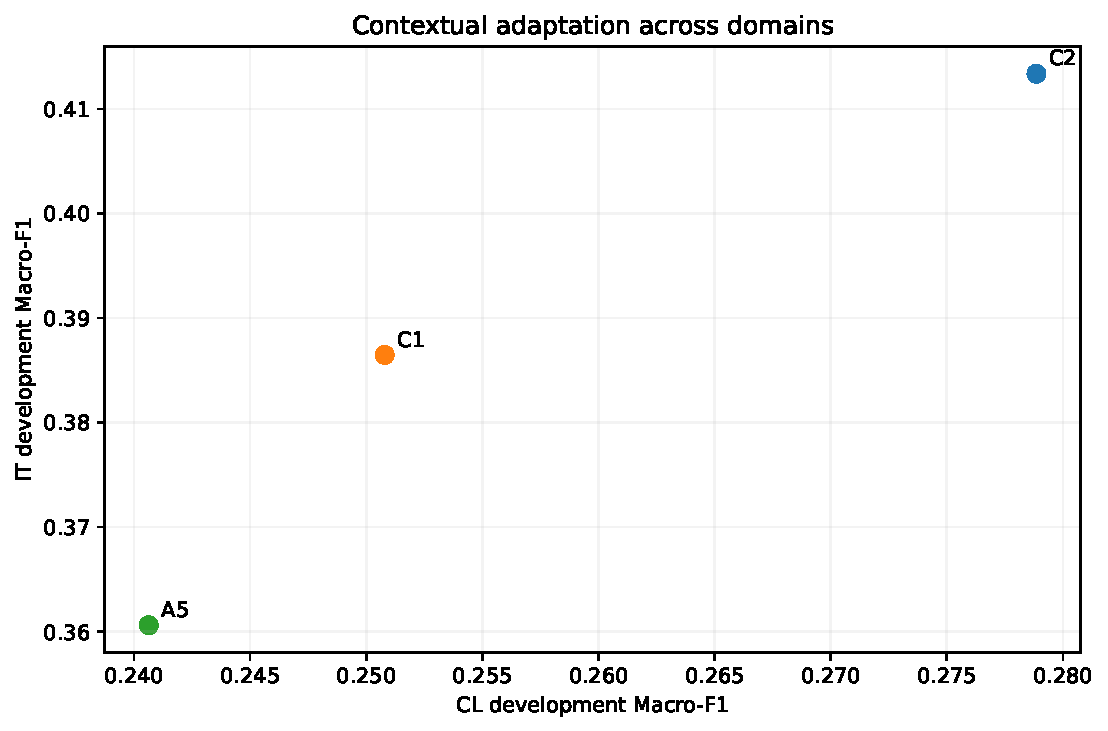
\includegraphics[width=.79\linewidth]{figures/phase3/p3_domain_comparison.pdf}
\caption{Development Macro-F1 by domain for baseline and local-context GQA. The official primary metric is pooled Macro-F1, not the arithmetic mean of the two domain scores.}
\label{fig:p3-domains}
\end{figure}

\subsection{Complete local and official results}
\label{sec:p3-results}
The notebook trained 16 independent classifier configurations. Two further candidate submissions were produced by postprocessing or combining trained outputs (C3 and D3), yielding 18 test archives. A local audit verified 10 required test-document IDs, 2,197 label predictions and exact allowed label names in every ZIP; this is a \emph{format and integrity} result, not proof that Codabench evaluated each one. The supplied screenshot shows 15 entries with a \method{Finished} score, one \method{Preparing}, and two \method{Failed}; two separate duplicate uploads for C2 and C3 were still \method{Submitting} at capture time.

\begin{longtable}{@{}r p{.44\linewidth} r r p{.14\linewidth}@{}}
\caption{Complete Phase-3 submission chronology. Development Macro-F1 is from the executed notebook and official Macro-F1 from the supplied Codabench screenshot. A numeric result in a Failed row is \emph{not} a confirmed completed evaluation. The D3 hybrid was not independently scored on development data.}\label{tab:p3-all}\\
\toprule
\# & Model or variant & Dev F1 & Official F1 & Status \\
\midrule\endfirsthead
\toprule
\# & Model or variant & Dev F1 & Official F1 & Status \\
\midrule\endhead
1 & A1\_\allowbreak decoder\_\allowbreak lora & 0.2934 & 0.3310 & Finished \\
2 & A2\_\allowbreak encdec\_\allowbreak lora & 0.1204 & 0.1361 & Finished \\
3 & A3\_\allowbreak prefix\_\allowbreak lora & 0.2350 & 0.2867 & Finished \\
4 & A4\_\allowbreak gqa100\_\allowbreak lora & 0.3073 & 0.3299 & Finished \\
5 & A5\_\allowbreak gqa700\_\allowbreak lora & 0.3291 & 0.3714 & Finished \\
6 & B1\_\allowbreak lorma\_\allowbreak plus & 0.3171 & -- & Failed \\
7 & B2\_\allowbreak ia3 & 0.2288 & -- & Preparing \\
8 & B3\_\allowbreak prefix & 0.1983 & 0.2379 & Finished \\
9 & B4\_\allowbreak full & 0.3330 & 0.4005 & Finished \\
10 & C1\_\allowbreak previous\_\allowbreak context & 0.3424 & 0.3976 & Finished \\
11 & \textbf{C2\_\allowbreak bidirectional\_\allowbreak context} & 0.3851 & \textbf{0.4249} & Finished \\
12 & C3\_\allowbreak document\_\allowbreak viterbi & 0.3527 & 0.3791 & Finished \\
13 & D1\_\allowbreak CL\_\allowbreak only & 0.2215 & 0.2586 & Finished \\
14 & D2\_\allowbreak IT\_\allowbreak only & 0.3020 & 0.3710 & Finished \\
15 & D3\_\allowbreak domain\_\allowbreak specialist\_\allowbreak hybrid & -- & 0.3957 & Finished \\
16 & E1\_\allowbreak student\_\allowbreak supervised & 0.3234 & 0.3679 & Finished \\
17 & E2\_\allowbreak student\_\allowbreak distilled & 0.3200 & 0.3638 & Finished \\
18 & F1\_\allowbreak balanced\_\allowbreak lora & 0.3459 & 0.3703 & Failed \\
\bottomrule
\end{longtable}


\begin{figure}[htbp]\centering
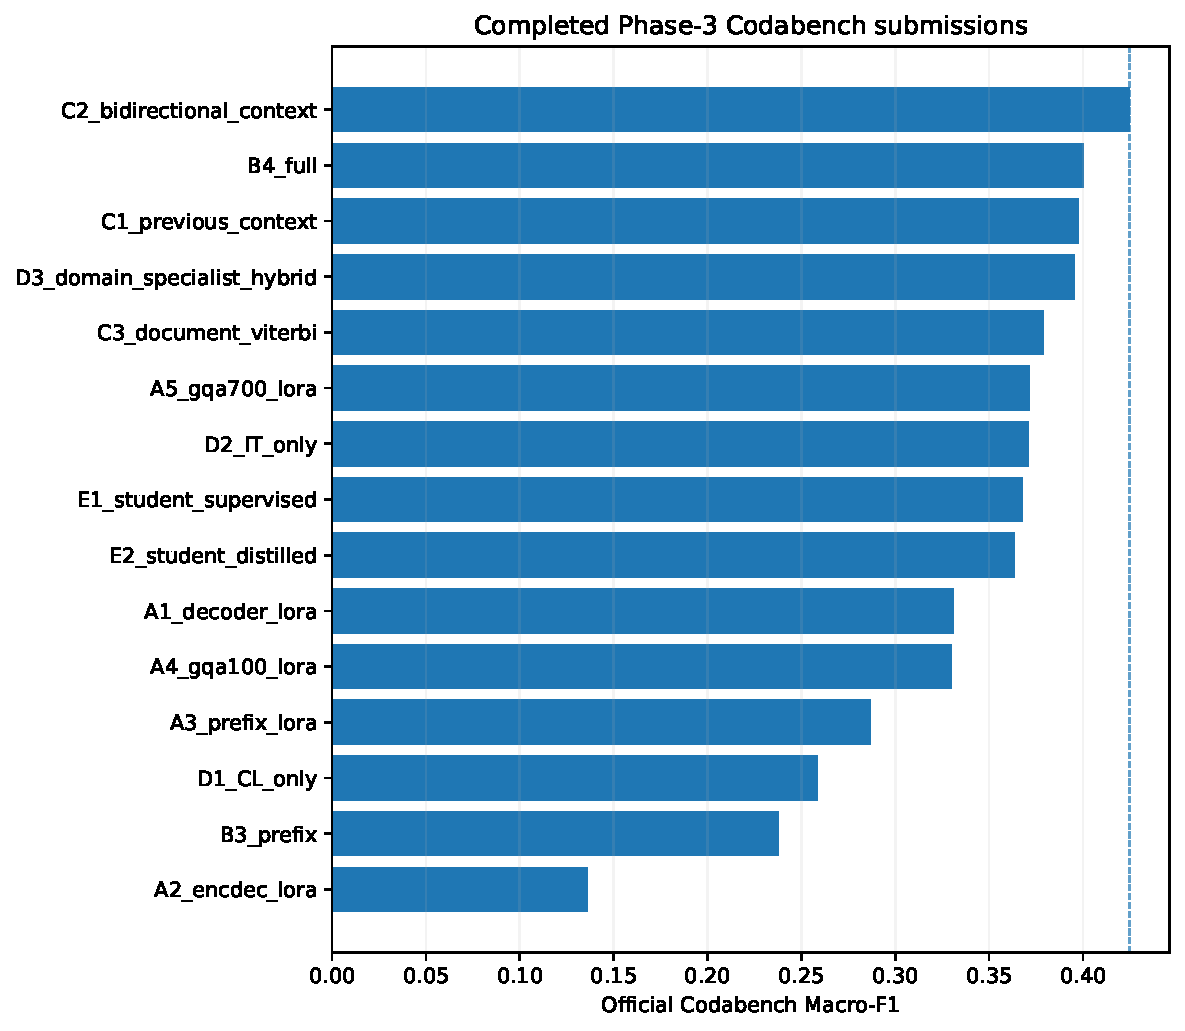
\includegraphics[width=.9\linewidth]{figures/phase3/p3_official_scores.pdf}
\caption{Official Phase-3 Macro-F1 for the 15 entries marked \method{Finished} in the supplied Codabench screenshot. Failed or pending rows are excluded even when a numeric value is visible.}
\label{fig:p3-official}
\end{figure}

\begin{figure}[htbp]\centering
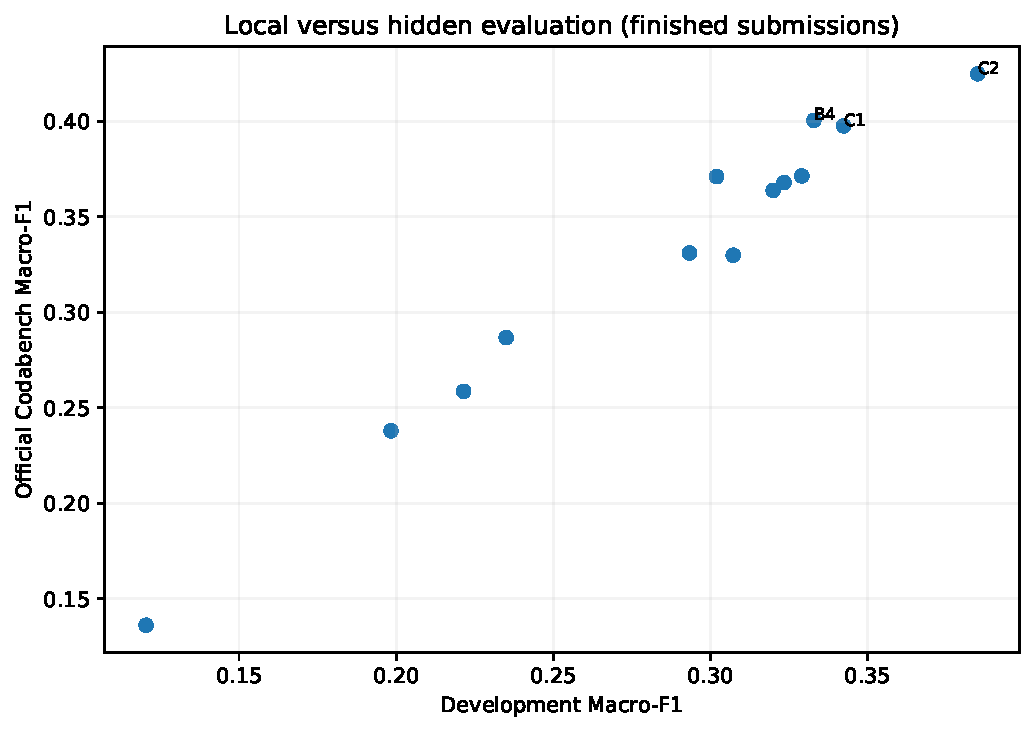
\includegraphics[width=.8\linewidth]{figures/phase3/p3_local_vs_official.pdf}
\caption{Notebook-selected local development F1 versus the official hidden-set primary metric for completed submissions with measured local scores. The plot makes the distinction between the two evaluation sources explicit.}
\label{fig:p3-local-official}
\end{figure}

The best confirmed official result is \textbf{C2 bidirectional-context GQA+LoRA, submission 989815, Macro-F1 0.4249}. By comparison, the same foundation and LoRA method without neighbors (A5) scored 0.3714, and the previous-sentence-only variant C1 scored 0.3976. The official C2--A5 gain is 0.0535 F1. C2 likewise led the local development analysis (0.3851), with the domain-wise development scores 0.2789 CL and 0.4134 IT. The official winner is selected by the private primary metric, not local training loss or larger trainable parameter count. We have no evidence of a numeric leaderboard rank and therefore report none.

\subsection{Error analysis and limitations}
\label{sec:p3-errors}
\begin{figure}[htbp]\centering
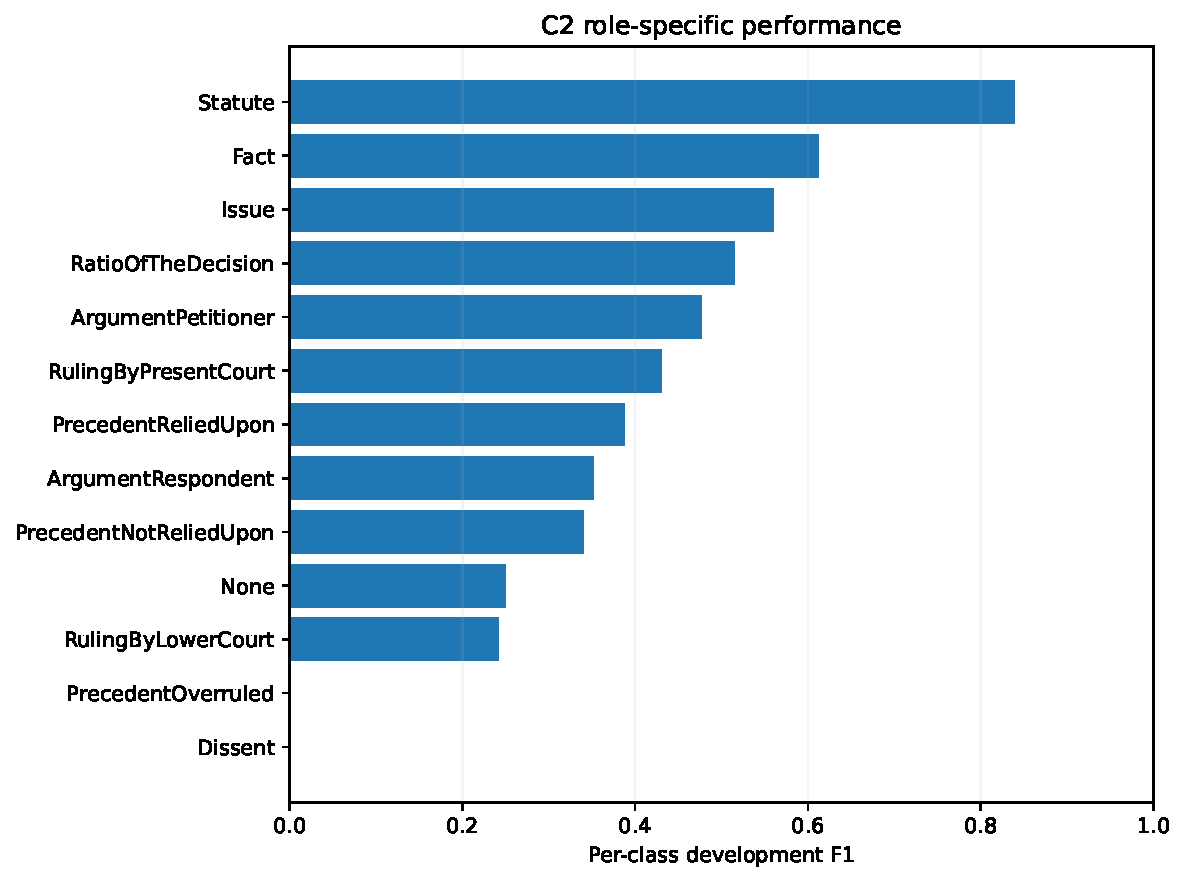
\includegraphics[width=.85\linewidth]{figures/phase3/p3_per_class_f1.pdf}
\caption{C2 development F1 for all 13 labels. The two classes absent from both development domains are scored zero by convention rather than treated as measured negative generalization cases.}
\label{fig:p3-classes}
\end{figure}

C2 produced development F1 0.839 for \method{Statute}, 0.613 for \method{Fact}, 0.560 for \method{Issue} (just 15 examples), 0.515 for \method{Ratio\allowbreak Of\allowbreak The\allowbreak Decision}, 0.352 for \method{Argument\allowbreak Respondent}, 0.242 for \method{Ruling\allowbreak By\allowbreak Lower\allowbreak Court}, and 0.250 for \method{None}. The strongest confusion in the saved error table was \method{Argument\allowbreak Petitioner} $\to$ \method{Ratio\allowbreak Of\allowbreak The\allowbreak Decision} (88 sentences), followed by \method{Precedent\allowbreak Relied\allowbreak Upon} $\to$ \method{Ratio\allowbreak Of\allowbreak The\allowbreak Decision} (81), \method{Fact} $\to$ \method{Ratio\allowbreak Of\allowbreak The\allowbreak Decision} (75) and \method{Argument\allowbreak Respondent} $\to$ \method{Ratio\allowbreak Of\allowbreak The\allowbreak Decision} (67). Other confusions included petitioner versus respondent arguments (46 in the petitioner-to-respondent direction and 60 in reverse) and lower-court ruling versus present-case reasoning (38 to \method{Ratio\allowbreak Of\allowbreak The\allowbreak Decision}). This pattern is consistent with difficulty separating reported legal positions from judicial reasoning, but it cannot prove the cause of any individual error without a contextual annotation audit.

The study is constrained by ten development judgments, uneven class support, one seed per central experiment and early stopping using the same small development set. Some comparisons change multiple factors: A1--A4 differ in pretraining objectives and pooling, and single-domain training changes both domain focus and the amount of available supervision. The 128-token cap and the 65\% target allocation in contextual runs truncate long sentences. There is no calibration or human expert review of ambiguous legal roles, no cross-domain held-out bootstrap interval, no direct paper-level claim of legal reasoning competence, and no independent validation of the official hidden labels. These limitations should be considered whenever interpreting differences of only a few F1 thousandths.

\subsection{Reproduction and winning-model handoff}
The clean research code is organized under \path{code/phase3/} and uses the existing \path{code/phase1/models.py} foundation definitions. It provides strict official JSON parsing, the original BPE token IDs, all adaptation methods, context building, native 13-class evaluation, resume-aware training, Viterbi decoding, hybrid composition, and strict ZIP validation. Local numeric evidence is retained in \path{code/phase3/experiments/}; the seven vector plots are regenerated from this evidence by \path{code/phase3/analysis/figures.py}. The best-model-only package is separate: it contains the exact GQA backbone, C2 attention LoRA, context encoding and inference routine, but not the research-only variants. Neither artifact includes pretrained weights, data or credentials.

The winning inference requires the preserved Phase-1 \path{best_up_to_700M.pt}, the Phase-3 \path{C2_bidirectional_context/best.pt} adapter/head state, and the original \path{legal_bpe_32k.json}. Validation of the archived original large backbone/adapter pair with regenerated bitwise-equivalent predictions remains pending where large remote checkpoint transfers are unavailable. Syntax tests, offline model smoke tests and format tests are valuable but cannot substitute for that final replay. The official hidden-test labels are not available and are not reconstructed.

\subsection{Conclusions and next research questions}
The Phase-3 study shows that compact, internally pretrained legal models are trainable for sentence-level rhetorical classification; the best measured improvement arose from \emph{neighboring-sentence context}, rather than a more expensive full fine-tune or a larger standalone head. Extended Phase-1 pretraining helped downstream local classification even though it did not improve Phase-1 hidden continuation BERTScore, illustrating task-dependent checkpoint value. Domain-only training was not competitive under the data available, and model compression improved measured throughput but did not improve F1 under this distillation objective. Further scientifically useful experiments would compare a hierarchical document encoder with the current causal context packing, apply document-level bootstrap intervals and multiple seeds, test calibrated rare-role handling, and isolate truncation effects on long judgments. None of these extensions is misrepresented as a completed Phase-3 experiment.


\section{Phase 4: Court Judgment Prediction}
\label{sec:phase4}

\subsection{Task and evaluation protocol}

The task assigns one of two outcome labels to each judgment in the course's
\path{Phase_4_CJPE} dataset. The primary metric is
$\mathrm{MacroF1}=(F_{1,0}+F_{1,1})/2$. The official test contains 1,517
judgments with hidden labels. Internal validation selected the checkpoint and
classification threshold. The clean development set served as a separate local
evaluation. A valid submission contains a single root-level
\path{prediction.json} with one string case ID and one binary integer prediction
per test judgment.

\begin{table}[htbp]
\centering\small
\caption{Rows, unique judgments and document lengths in the original files.
Word statistics describe rows before case-level deduplication.}
\label{tab:p4-data}
\begin{tabular}{lrrrrr}
\toprule
Split & Rows & Unique IDs & Median words & 95th percentile & Maximum words \\
\midrule
Train & 37,387 & 32,305 & 2,192 & 9,195 & 412,606 \\
Dev   & 1,988  & 994    & 2,822 & 9,280 & 42,198 \\
Test  & 1,517  & 1,517  & 2,940 & 10,023 & 40,487 \\
\bottomrule
\end{tabular}
\end{table}

The case audit found repeated IDs in 5,082 training cases and 994 development
cases. Those repeated IDs had identical normalized text and consistent labels.
The pipeline keeps the longest available text per ID with stable tie handling.
It removes development rows that share an ID or a lowercase, whitespace-normalized
text hash with test. The saved audit found zero such overlaps. A ten-fold
stratified group split (seed 42) grouped identical texts and selected the fold
closest to a 10\% holdout and the original positive-class proportion. This
yielded 29,074 training and 3,231 internal validation cases, each with about
41.4\% class 1. Clean development has 497 cases per class. A constant-class
predictor obtains 0.5000 accuracy and 0.3333 macro-F1 on that split.

\subsection{Representations and experimental design}

The tokenizer is the original 32,000-token Phase-1 byte-level BPE. The single
window retains the last 1,022 content tokens with BOS and EOS and right-padding
to at most 1,024 tokens. Tail sampling prioritizes the portion of the judgment
where dispositions may appear. It can omit facts, precedent, or procedural
context earlier in a long document. A head-and-tail representation was
prepared and checked. All eight trained runs used the tail or hierarchical
representation, so no separate head-and-tail score is available.

\begin{description}[leftmargin=1.4em]
\item[E01.] Full fine-tuning of the 700,047,360-token Efficient GQA
  foundation (14 blocks, 768 hidden units, 12 query and 4 key/value heads).
  A dropout and linear head classify the final non-padding state. The
  resulting model has 112,680,194 parameters.
\item[E02.] Up to five evenly spaced windows, always including the tail, are
  encoded with frozen E01 weights. Their final-token vectors and logits are
  cached in float16. A position-aware attention head pools chunk vectors.
  Its learned correction uses the pooled vector, tail vector, and their
  difference, then adds two residual logits to the original tail logits.
  The zero-initialized final layer starts at the frozen tail decision.
\item[E03.] Output-space multiplicative LoRMA+ with rank 16 and scale
  $\alpha/r=32/16$ in the four GQA projections and three SwiGLU projections
  per block. The pretrained matrix remains frozen and the adapter adds
  $(\alpha/r)BA(W_0x)$ to its output before bias.
\item[E04--E06.] Full tuning of the original 100,024,320-token causal decoder,
  Prefix-LM, and encoder--decoder. The decoder pools the final non-padding
  state. Prefix-LM exposes the whole valid prefix bidirectionally and masks
  padding. The encoder--decoder uses one BOS decoder query over masked
  encoder memory, with padding excluded from encoder and cross-attention.
\item[E07.] Adaptive-rank GQA freezes the same 700M foundation and adapts
  56 attention projections with a masked rank-16 factorization. An
  exponential moving average of gradient sensitivity guides irreversible
  pruning every 40 optimizer updates. The cubic budget schedule targets
  mean rank 8 with at least 2 active components per projection. The
  archived run decreased from 896 to 448 active components.
\item[E08.] A six-layer causal Transformer (384 hidden units, six heads,
  23,329,538 parameters) learns from E01 logits and the true labels.
  The objective is $0.35\,\mathrm{CE}+0.65\,T^2
  \mathrm{KL}(p_{\mathrm{teacher},T}\Vert p_{\mathrm{student},T})$ with $T=2$.
  This is about a 4.83-fold reduction in parameters relative to E01.
\item[E09--E10.] Probability blends pair E01 with E05 and E08 respectively.
  Nine E01 weights in $[0.55,0.95]$ and 51 thresholds in $[0.25,0.75]$ are
  searched on internal validation. Both selected an E01 weight of 0.90.
\end{description}

Full tuning used AdamW with backbone and head learning rates of
$2\times10^{-5}$ and $3\times10^{-4}$, microbatches of eight, four accumulation
steps, gradient clipping at 1.0, and 6\% warmup followed by cosine decay
with a 5\% floor. Adapter and student schedules retain their recorded
run-specific rates and batch sizes. E02 trains only the residual head and
uses a constant $2\times10^{-4}$ learning rate with batch size 256. The
checkpoint criterion was internal macro-F1 at threshold 0.50. Thresholds
for single runs were then tuned on the selected checkpoint's internal
predictions, preferring the threshold closest to 0.50 on a tie.
Figure~\ref{fig:p4-history} plots pre-calibration scores. These differ
from the calibrated scores in Table~\ref{tab:p4-scores}.

\begin{figure}[htbp]
\centering
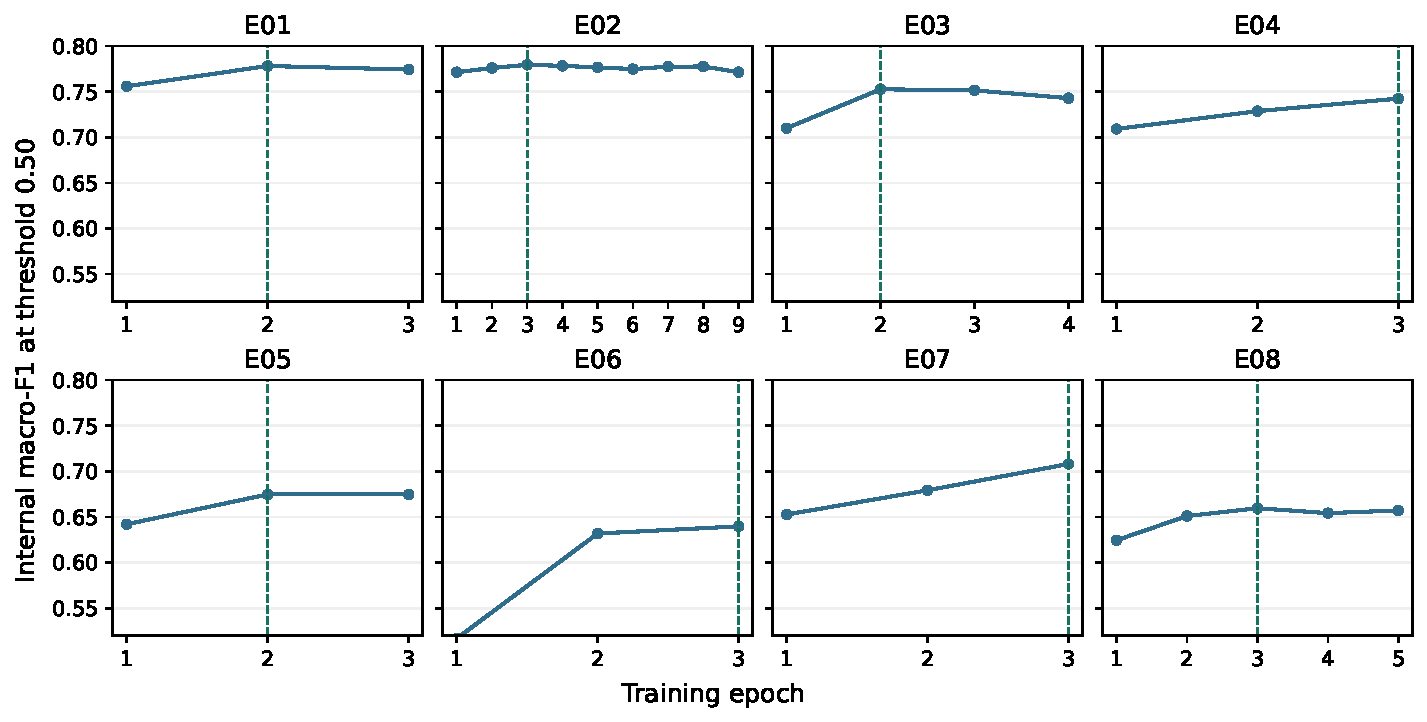
\includegraphics[width=\linewidth]{figures/phase4/p4_validation_history.pdf}
\caption{Saved epoch histories for all eight trained runs. The dashed line
marks the selected checkpoint. E02 starts from frozen E01 features, and
E08 starts from a newly initialized student, so the trajectories represent
different training regimes.}
\label{fig:p4-history}
\end{figure}

\subsection{Results and error analysis}

\begin{table}[htbp]
\centering\small
\caption{Macro-F1 by split at the selected threshold. The official scores
are supplied Codabench results. Internal and clean development scores
were recomputed from the saved outputs.}
\label{tab:p4-scores}
\begin{tabular}{llrrrr}
\toprule
Run & Experiment & Threshold & Internal & Clean dev & Codabench \\
\midrule
E01 & Efficient GQA full tuning & 0.51 & 0.7795 & 0.7328 & \textbf{0.7393} \\
E02 & Hierarchical GQA & 0.45 & 0.7809 & 0.7233 & 0.7263 \\
E03 & GQA LoRMA+ & 0.49 & 0.7548 & 0.6576 & 0.6749 \\
E04 & Decoder-only full tuning & 0.50 & 0.7423 & 0.6911 & 0.6976 \\
E05 & Prefix-LM full tuning & 0.49 & 0.6769 & 0.6445 & 0.6476 \\
E06 & Encoder--decoder full tuning & 0.46 & 0.6480 & 0.6133 & 0.6013 \\
E07 & Adaptive-rank GQA & 0.44 & 0.7150 & 0.6394 & 0.6580 \\
E08 & Distilled Transformer & 0.47 & 0.6643 & 0.6015 & 0.6126 \\
E09 & GQA + Prefix-LM & 0.48 & 0.7797 & 0.7346 & 0.7353 \\
E10 & GQA + distilled student & 0.49 & 0.7797 & 0.7329 & 0.7369 \\
\bottomrule
\end{tabular}

\end{table}

\begin{figure}[htbp]
\centering
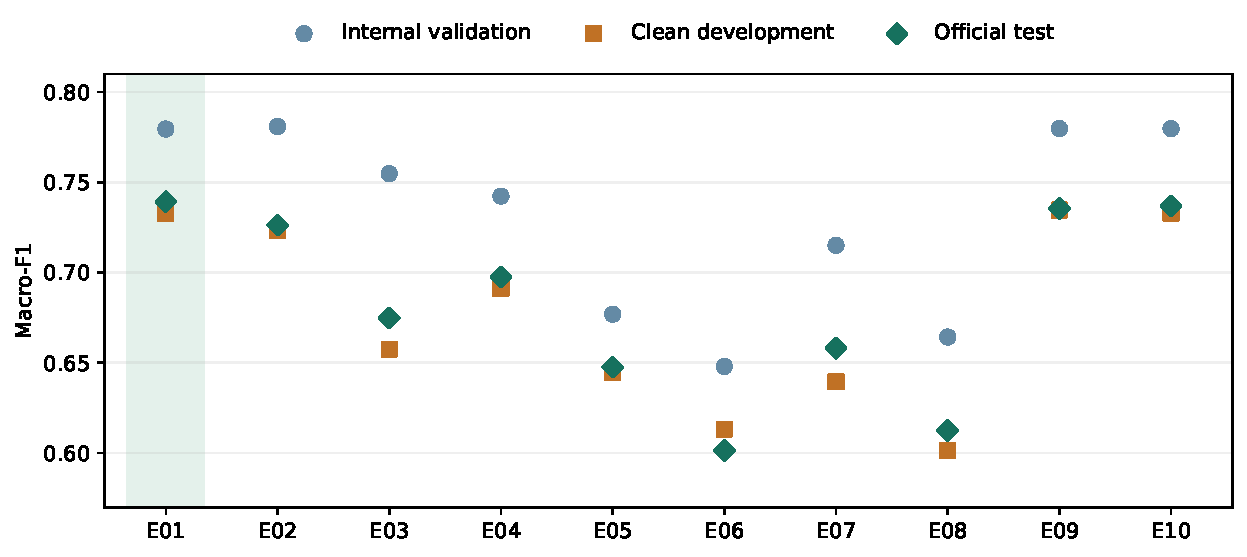
\includegraphics[width=\linewidth]{figures/phase4/p4_split_scores.pdf}
\caption{Local and official scores for all ten submissions. E02 leads on
internal validation and E09 leads on clean development. E01 leads on the
official test.}
\label{fig:p4-scores}
\end{figure}

E01 achieved the best recorded official macro-F1 of \textbf{0.7393}, ahead
of E10 (0.7369) and E09 (0.7353) by 0.0024 and 0.0040. E09 improved on E01
by 0.0018 on clean development but fell behind on the official test.
E02 improved internal macro-F1 from 0.7795 to 0.7809 while trailing E01
on both development and test. Extra document coverage and the learned
residual therefore did not yield a consistent improvement under the
observed protocol.

Among full-tuning runs, E04, E05 and E06 scored 0.6976, 0.6476 and 0.6013
officially. E01 differed in both architecture and pretraining exposure,
so the comparison cannot isolate the effect of grouped-query attention.
E03 and E07 started from the same 700M foundation as E01, but changed
the objective's trainable parameterization, optimization settings and
training schedule. E08 reached 0.6126 officially with substantially
fewer parameters. The experiment did not train a same-size supervised
student as a control, leaving the marginal effect of distillation
unmeasured.

\begin{figure}[htbp]
\centering
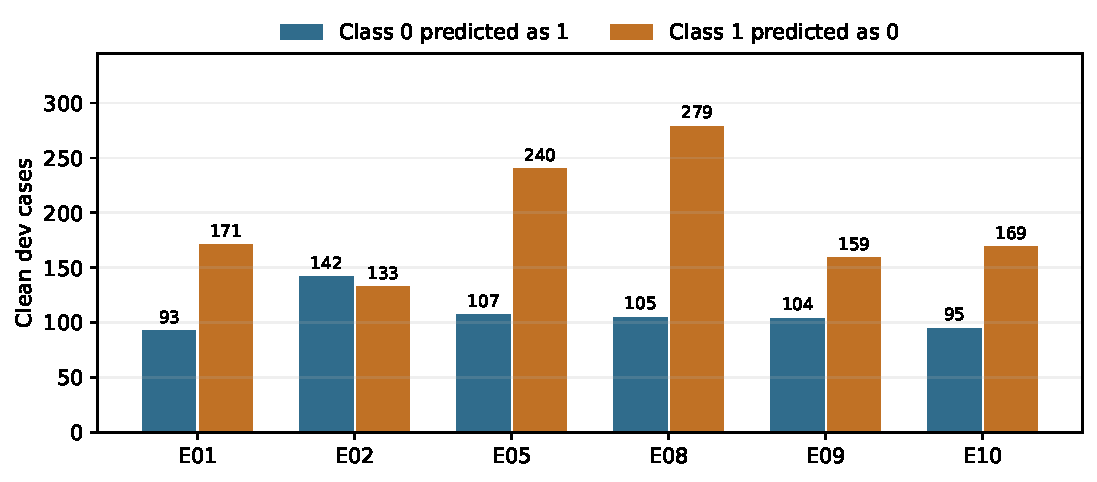
\includegraphics[width=.92\linewidth]{figures/phase4/p4_dev_errors.pdf}
\caption{Selected clean development error counts at each run's chosen
threshold. The clean split contains 497 cases per class.}
\label{fig:p4-errors}
\end{figure}

At its selected threshold E01 missed 171 of 497 class-1 cases and
classified 93 of 497 class-0 cases as class 1. E02 reduced the first
error to 133 while increasing the second to 142, a tradeoff consistent
with its lower threshold and altered scoring model. E09 made 12 fewer
class-1 misses and 11 more class-0 errors than E01 on clean development.
E08 missed 279 class-1 cases and had class-1 F1 of 0.5317. These are
aggregate observations on labeled local data. The test labels are hidden.
Differences of a few thousandths between E01 and the blends are point
estimates from single executions. The study did not quantify seed
variation or official-test uncertainty.

\subsection{Reproduction and verification}

The released CLI prepares case splits and token caches, trains with
optimizer-step resume, evaluates checkpoints and exports validated
archives. It also rebuilds the blends from aligned saved member scores
and teacher logits. All ten archived submissions were checked against the
official test IDs. All ten label sets were reproduced from saved scores or
logits, and both ensemble searches recovered the recorded weights and
thresholds. The separate E01 source package uses the saved epoch-2
checkpoint and the fixed 0.51 threshold. Full GPU training replay and
original E01 weight inference remain open. The available Drive transfer
route rejected the 450,775,315-byte E01 checkpoint. Checkpoint and
numerical verification details are in the Phase-4 README.

\clearpage
\section{Phase 6: Legal Abstractive Summarization}
\label{sec:phase6}

\subsection{Task, constraints and evaluation}
The system receives a judgment and must compress its material facts, legal
reasoning and disposition into a readable abstraction. Given a document
\(d\) and output tokens \(y_{1:m}\), a conditional generator models
\[
 p_\theta(y_{1:m}\mid d)=\prod_{t=1}^{m}p_\theta(y_t\mid d,y_{<t}).
\]
For long cases the submitted system applies this factorization separately to
selected passages of \(d\), then orders and merges their outputs. This trades
whole-document context for multiple bounded generation calls. An abstraction
can paraphrase beyond source sentences, so factual support and lexical overlap
are separate questions. See \href{https://arxiv.org/abs/1904.09675}{Zhang et al. on BERTScore}.

The course required adaptation of all four Phase~1 architectures, including
LoRMA and a smaller distilled model. Training was confined to the course
dataset and the project's own Phase~1 weights. The official configuration,
\path{Phase_6_Summ}, provides \path{Train/train.json} and \path{Test/test.json}.
The labeled records contain an ID, judgment and summary. Test references are
hidden, and the course publishes no separate development split. Each submitted
archive contains a root-level \path{prediction.json} with an ID and a nonempty
summary per test judgment. The course specifies \BERT{} as the primary measure
and ROUGE-1/ROUGE-L F1 as secondary measures. The available official result
record contains the primary scores and submission IDs. Local results are
mean stemmed ROUGE F1 over held-out judgments and are reported separately.

\subsection{Data and the context constraint}
Of 7,030 labeled records, 6,466 went to training and 564 to validation. A
grouped split uses SHA-256 of whitespace-normalized source text to keep exact
duplicates together. The archived partition is authoritative for replay.
The 100 test judgments were reserved for submission. The original notebook
reports a median of 17,905 source characters, rising to 45,052 at the 90th
percentile. References have a median of 638 words, a 90th percentile of
1,501 and a maximum of 27,768. Two training references are empty.
The original 240-token target cap includes the end-of-sequence token and
already binds at the median training example. The original and revised
methods therefore solve substantially different supervision problems.

\begin{figure}[!htb]
\centering
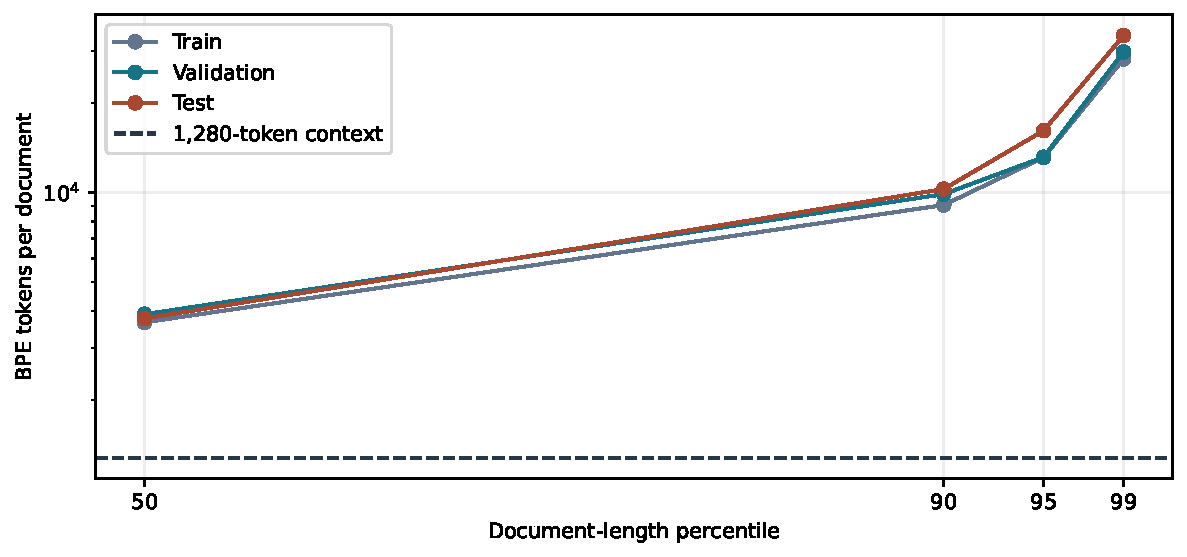
\includegraphics[width=.84\linewidth]{figures/phase6/p6_data_lengths.pdf}
\caption{Document length quantiles obtained with the archived 32k Phase~1
byte-level BPE tokenizer. The dashed line marks the causal context budget
before accounting for prompt or output tokens.}
\label{fig:p6-lengths}
\end{figure}

The split-level measurements in Table~\ref{tab:p6-lengths} show that even
the median document is almost three times the causal context. The training
reference itself has a median of 753 BPE tokens, beyond either target cap.
The 99th-percentile training source has 28,190 BPE tokens, with a maximum of
162,070. The median within-case document-to-summary ratio is 4.59:1 for
nonempty training references and 4.65:1 in validation. The labeled file
contains 27 extra rows beyond its number of normalized-text groups. No
labeled and test IDs or exact normalized sources overlap. Exact hashing
does not detect edited near duplicates.

\begin{table}[!htb]
\centering\small
\caption{Median source and reference lengths. Source thresholds use the 1,280-token
causal context before prompt or output tokens. Test references are private.}
\label{tab:p6-lengths}
\begin{tabular}{lrrrrr}
\toprule
Split & Count & Source words & Source BPE & Over context & Ref. words \\
\midrule
Train & 6,466 & 3,120 & 3,657 & 94.4\% & 638 \\
Validation & 564 & 3,353 & 3,893 & 93.1\% & 647 \\
Test & 100 & 3,171 & 3,768 & 95.0\% & -- \\
\bottomrule
\end{tabular}
\end{table}

\subsection{Inputs, alignment and training coverage}
\paragraph{Original section packing.}
The notebook divides a long judgment into 150-token sections, prioritizes the
first and last two sections, then ranks the remaining sections by legal-term
frequency with a small bonus for later position. It concatenates the selected
sections in source order under a nominal 900-token text budget, with a single
instruction and summary cue. The target takes up to 239 BPE tokens and appends
EOS, even if the last reference sentence is incomplete. The training cache
contains one pair per judgment. A head-only comparator replaces the section
selection with the initial source span. The method packs discontiguous
evidence into one context and gives the model a single output budget.

\paragraph{V2 passage alignment.}
The revisions use contiguous 840-token windows. The first and last windows
are mandatory, with up to two interior windows chosen by legal-term frequency
and a decision-cue bonus. The prompt labels each selected passage by its
position among the selected passages. During training, for each reference
sentence \(s\) and passage \(p\) the assignment score is
\[
 a(s,p)=\frac{|W(s)\cap W(p)|}{\max(1,\sqrt{|W(s)||W(p)|})},
\]
where \(W\) is the set of lowercased content words and eligible numerals.
The best passage receives the sentence if its score reaches 0.05. V2 forms
one target of up to 319 tokens plus EOS per eligible passage, preferring
high-overlap sentences when the assigned text exceeds the budget. Selection
for inference depends only on the source. The cache has 21,710 training
passage examples across 6,464 usable judgments and 1,897 validation passages.
Each epoch rotates one passage per judgment, yielding 19,392 draws over
three epochs with repeated passages on shorter cases and omissions for
cases with four targets.

\paragraph{V3 target packing.}
V3 preserves the order of all aligned sentences and opens a new target pack
when the next sentence would exceed the cap. It tries clause boundaries for
overlong sentences and skips fragments that still cannot fit. Sentences
without a qualifying passage remain outside the training targets. V3 draws
31,668 packed targets, or 4.9 per usable training judgment, plus 2,778
validation targets. The 50th, 90th and 99th percentiles of training target
length including EOS are 212, 309 and 319. Each run shuffles judgments,
shuffles their target packs and visits all packs once, resulting in 7,917
optimizer updates. The evidence establishes complete coverage of the
materialized target set.

\subsection{Backbones, parameter updates and objective}
All adaptations reuse the Phase~1 32k BPE, with PAD, BOS, EOS and UNK at IDs
0 through 3. The GQA runs start from the 700M-token foundation. The other
backbones use their Phase~1 best snapshots. The encoder--decoder attends
bidirectionally to an input of up to 1,024 tokens, and generates with a
causal decoder of capacity 640 with cross-attention. Prefix-LM processes its
source prefix bidirectionally and continues causally, within 1,280 tokens.
The standard decoder uses causal self-attention and learned positional
embeddings. Efficient GQA is causal with fourteen 768-wide blocks, twelve
query and four KV heads, rotary position embeddings, RMS normalization and
SwiGLU. See \href{https://aclanthology.org/2023.emnlp-main.298/}{Ainslie et al. on grouped-query attention}. The GQA LoRA run trains 3.06M of its 115.72M parameters in V3.

\begin{itemize}[leftmargin=*]
\item E01 and E05 test additive low-rank adaptation on encoder--decoder and
Efficient GQA. A frozen projection \(W\) receives the trainable update
\(Wx+(\alpha/r)BAx\).
\item E02 tests the notebook's LoRMA+ multiplicative form. If \(z=Wx\), the
layer returns \(z+(\alpha/r)BAz\). Its low-rank factors operate in the
projection's output space.
\item Original low-rank adapters have rank 8 and scale \(\alpha/r=2\).
They target selected attention projections. V2/V3 use rank 16 and the same
scale, expand adaptation to attention and MLP linears, and train the
normalization parameters.
\item E03 tests a prefix-conditioned source with residual adapters. The
original attaches a normalized width-64 ReLU adapter after the block.
V2/V3 insert separate bottlenecks after attention and the MLP and also train
the layer norms. Up-projections start at zero.
\item E06 trains all 101.97M encoder--decoder parameters. E04 and E07 train
all 82.26M parameters of an eight-layer causal student assembled from layers
0, 2, 3, 5, 6, 8, 9 and 11 of the Phase~1 standard decoder.
\end{itemize}

The adaptation designs follow
\href{https://arxiv.org/abs/2106.09685}{Hu et al. on LoRA},
\href{https://arxiv.org/abs/2506.07621}{the LoRMA paper} and
\href{https://proceedings.mlr.press/v97/houlsby19a.html}{Houlsby et al. on adapters}.
The formulas above describe this project's implemented variants.

Teacher forcing minimizes mean target-token cross-entropy
\[
 \mathcal L_{\mathrm{CE}}=-\frac{1}{|y|}\sum_{t=1}^{|y|}
 \log p_\theta(y_t\mid x,y_{<t}).
\]
EOS is supervised. Decoder-only and prefix models use logits starting at the
last prompt position, masking source positions out of the loss by slicing.
The encoder--decoder sees the source in the encoder and BOS followed by
shifted gold tokens in its decoder. Microbatches contain one example, avoiding
padding masks. The optimizer is AdamW with weight decay 0.01, accumulation
over four examples and gradient clipping at 1.0. The notebooks use mixed
precision, warm-up and cosine decay. Original updates range from 500 to
800. V2 uses 4,848 updates per run. V3 uses one complete 7,917-update pass.
Learning rates decrease from \(2\cdot10^{-4}\) for original adapters, to
\(1.5\cdot10^{-4}\) for V2 and \(8\cdot10^{-5}\) for V3. Full fine-tuning
uses \(2\cdot10^{-5}\) in original/V2 and \(10^{-5}\) in V3.
Student rates are \(4\cdot10^{-5}\) in original/V2 and \(2\cdot10^{-5}\) in V3.

\subsection{Teacher and student comparison}
E02 was the teacher in each version. The original selects the teacher by
held-out ROUGE-L and generates responses for 1,000 documents. V2 selects
by hierarchical ROUGE-1 and stores 2,686 generated passage responses from
800 selected judgments. In both, approximately half of E04's scheduled draws
are replaced by draws from the teacher-labeled pool. For examples with a
pseudo-target, the original mixes gold and teacher-sequence CE equally.
V2 uses a 60:40 gold-to-teacher mixture. V2 E04 reaches 0.3160 local ROUGE-1
against 0.3976 for its gold-only counterpart.

V3 uses the V2 gold-only checkpoint as the initialization for both E04 and
E07. The larger frozen E02 teacher receives the same gold target prefix as
the student and computes the vocabulary distributions online. With
\(p_T\) the teacher distribution and \(q_T\) the student distribution at
temperature \(T=2\), the loss is
\[
  \mathcal L_{\mathrm{V3,E04}} =
  0.8\,\mathcal L_{\mathrm{CE}}+
  0.2\, T^2\,\frac{1}{|y|}\sum_{t=1}^{|y|}
  D_{\mathrm{KL}}\!\left(p_T(\cdot\mid x,y_{<t})
        \,\|\,q_T(\cdot\mid x,y_{<t})\right).
\]
E07 uses gold CE alone. The controls share architecture, warm start, budget
and coverage. Run-specific shuffles differ. E04 improves held-out NLL over
E07 (2.3575 versus 2.3768), while E07 leads it by 0.0259 in validation
ROUGE-1 and 0.0017 in official \BERT{}. The data support the outcome of this
one teacher, temperature and mixture with their observed shuffles. The
smaller V3 ROUGE gap relative to V2 is descriptive, since data construction,
training budget and evaluation sample changed.

\subsection{Decoding, selection and results}
Original cached greedy decoding blocks PAD, BOS, UNK and repeat trigrams,
uses a repetition penalty of 1.12 and allows EOS after 40 generated tokens,
with a 192-token cap. V2/V3 use 1.10, 32 and 260 respectively, per selected
passage and within context capacity. They trim a trailing incomplete segment
when the last terminal punctuation is at or after 65\% of the generated
text, then combine passages in document order. Sentence deduplication drops
later candidates with content-word Jaccard overlap above 0.73. This merge
preserves more separate source evidence and can retain contradictions across
passages.

V3 compares raw merging with an optional lexical filter. A sentence must
share at least 52\% of its eligible words with the source and any matched
multi-digit number must occur in the source text. If fewer than 30 words
survive deduplication, it falls back to the raw summary. All seven V3
experiments selected raw based on held-out ROUGE-1. For E05 the filter
reduces mean length from 295 to 273 words and ROUGE-1 from 0.4092 to
0.3931. This proxy can remove valid paraphrases and retain reversed legal
relationships with shared vocabulary.

\begin{figure}[!htb]
\centering
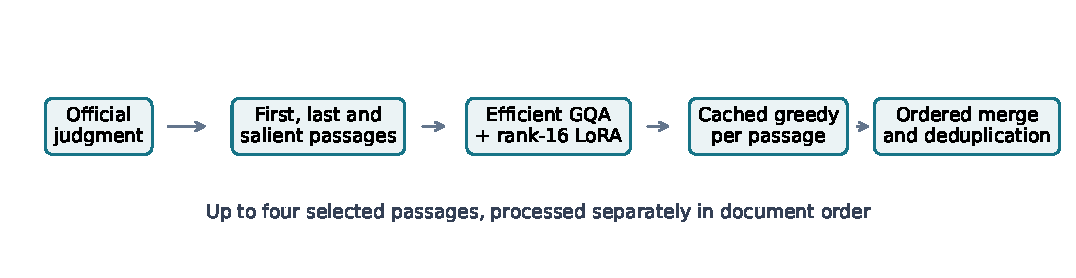
\includegraphics[width=.97\linewidth]{figures/phase6/p6_e05_pipeline.pdf}
\caption{Submitted E05 inference. Passage selection precedes cached generation.
The raw policy orders and deduplicates generated sentences.}
\label{fig:p6-pipeline}
\end{figure}

\begin{table}[!htb]
\centering\small
\caption{V3 held-out and official results. Local scores use 96 documents.
Official scores use 100 hidden-reference cases. IDs and scores are transcribed
from the supplied Codabench screenshot and mapped by the submission order.}
\label{tab:p6-official}
\begin{tabular}{llrrrrr}
\toprule
Run & Method & Best step & ROUGE-1 & ROUGE-L & \BERT{} & ID \\
\midrule
E01 & Enc.--dec. LoRA & 7,917 & .2504 & .1602 & .8217 & 1026549 \\
E02 & GQA LoRMA & 7,917 & .4129 & .2278 & .8442 & 1026551 \\
E03 & Prefix Houlsby & 7,750 & .2847 & .1764 & .8239 & 1026552 \\
E04 & Causal student KL & 7,750 & .3975 & .2198 & .8438 & 1026554 \\
E05 & GQA LoRA & 7,750 & .4092 & .2236 & \textbf{.8459} & 1026556 \\
E06 & Enc.--dec. full & 7,917 & .2686 & .1661 & .8232 & 1026558 \\
E07 & Causal student CE & 7,500 & \textbf{.4234} & \textbf{.2310} & .8455 & 1026559 \\
\bottomrule
\end{tabular}
\end{table}

\begin{figure}[!htb]
\centering
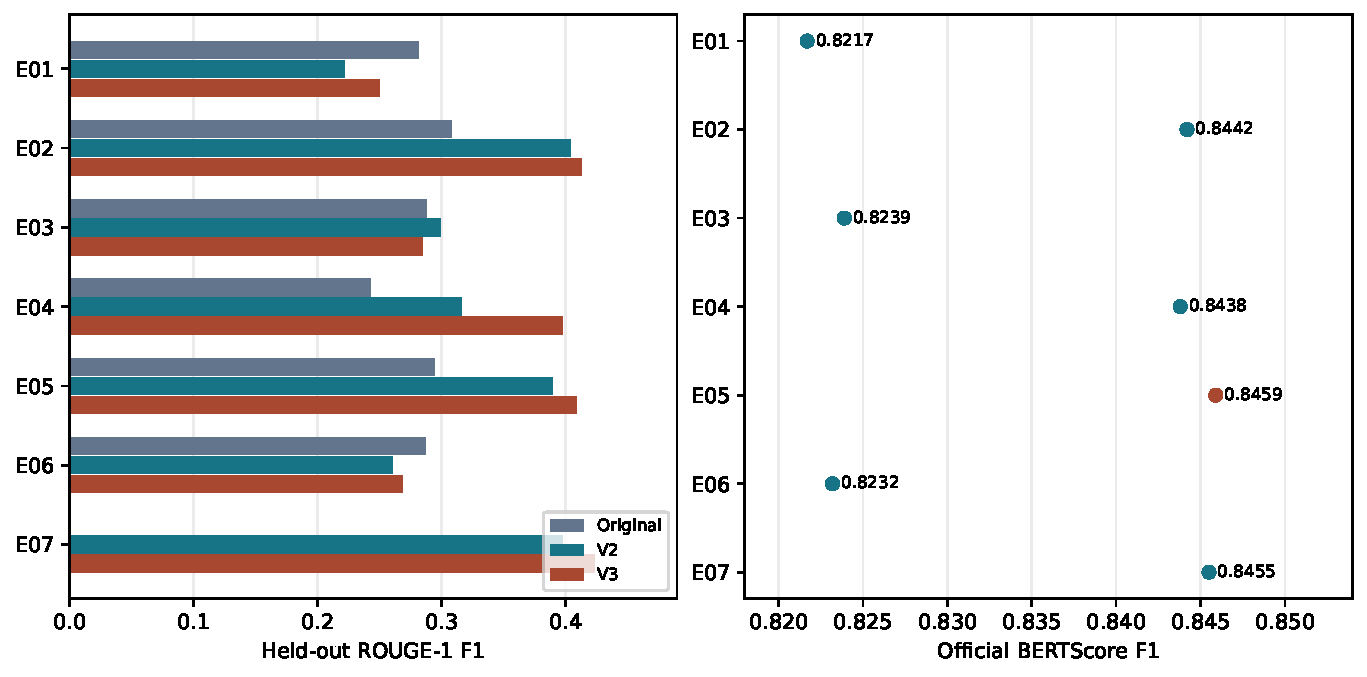
\includegraphics[width=.98\linewidth]{figures/phase6/p6_results.pdf}
\caption{Local lexical performance by revision and official V3 BERTScore F1.
Local samples contain 32, 64 and 96 judgments across the three revisions.
The two panels use different metrics and evaluation cases.}
\label{fig:p6-results}
\end{figure}

\begin{figure}[!htb]
\centering
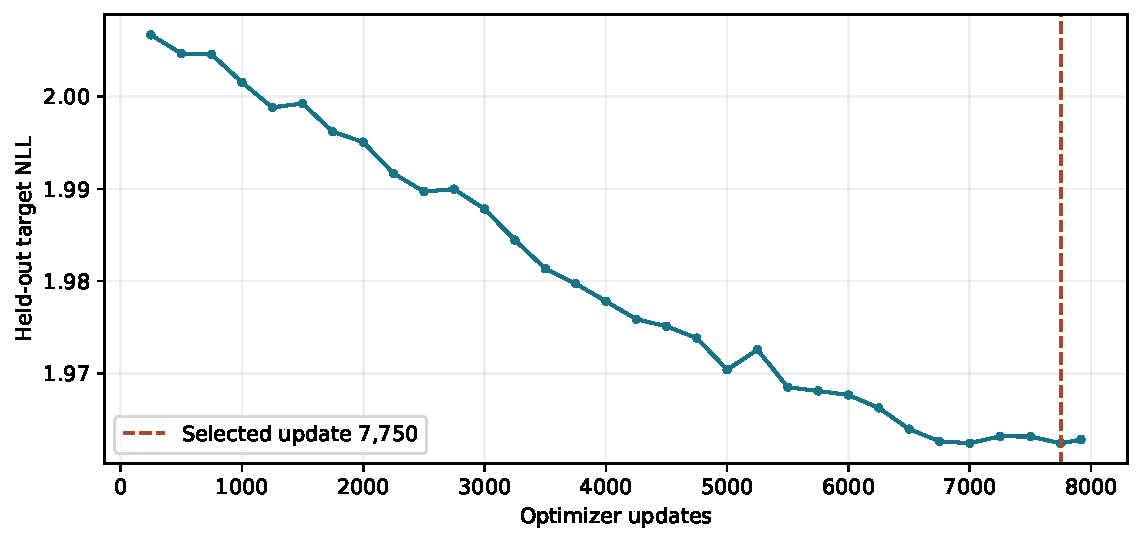
\includegraphics[width=.83\linewidth]{figures/phase6/p6_e05_history.pdf}
\caption{Archived V3 E05 target NLL on the fixed validation subset.
The archive selected update 7,750. Several late values look close at the
displayed precision. The selected update comes from the submission manifest.}
\label{fig:p6-history}
\end{figure}

\paragraph{Long-case ablation.}
On V2's matched 64 judgments and E02 weights, head-only decoding gives
0.1797 ROUGE-1 and hierarchical decoding 0.4042. With V3's matched 96
judgments, the raw scores are 0.1860 and 0.4129. In V3 the mean output
length also increases from 98 to 302 words. The comparison changes both
source access and the number of possible generation calls. It does not
isolate salience, document coverage or length as causes.

\paragraph{What changed across runs.}
Original E02 led its local comparison at 0.3081 ROUGE-1. V2's better
document coverage and revised supervision gave the GQA and distilled runs
higher measured ROUGE, while encoder--decoder runs moved in the opposite
direction on the changed validation sample. V3 added more supervision
per selected passage and resumed the V2 models. E03's V3 lexical scores
declined relative to V2, even with the larger passage schedule. On the V3
official set the two GQA adapters and two causal students scored between
0.8438 and 0.8459. E01, E03 and E06 scored from 0.8217 to 0.8239. Initialization,
attention structure and trainable layers differ, so this ranking cannot
isolate an architecture or adaptation effect. E05 is the official winner
among the seven project submissions. Its 0.0004 advantage over E07 does
not establish a generalization advantage without paired scores or repeat
runs.

\subsection{Qualitative errors and scope of verification}
In archived V2 E02 validation output for judgment 1770, the generated
text adds Section 307 alongside Section 302 and changes the account of the
appellate reasoning relative to the reference. In judgment 757, the
prediction introduces a \pounds2,000 figure absent from the reference
account of the pension arrangement. These examples show how legal-sounding
details can diverge from reference facts. The analysis is illustrative and
does not estimate error prevalence or prove absence from every source
passage. A candidate may also copy a correct number in the wrong role,
or omit the disposition if the selected windows or generation budgets
discard it.

The evidence audit validates the archived submissions against the official
test IDs, recomputes available held-out metrics from saved predictions and
checks the selected run against the V3 manifest. Model and optimizer tests
exercise the port on synthetic weights. The original E05 checkpoint exceeds
the available Drive transfer limit. Original-weight decoding, full GPU
training and private score recomputation remain outside the verification
performed here.

\subsection{Conclusion}
The best recorded official summary system combines Phase~1 Efficient GQA
with a small trainable LoRA component and reference-independent passage
selection. Multiple generation calls recover more lexical coverage than a
single head window in matched comparisons. The distilled student remained
competitive, but its gold-only control scored higher on both generated
validation summaries and the hidden test. For legal use, the archived
errors motivate separate factual checks beyond the primary metric.


\appendix
\section{Supplementary Reproduction Notes}
\subsection{Experiment ledger and provenance}
The repository's \method{code/phase1/experiments/official\_and\_local\_results.csv} records all seven submitted variants, their official primary and secondary metrics, training budget, decoding configuration, model size and locally available metrics. The \method{validation\_curve.csv}, \method{decoding\_sweep.csv}, and \method{full\_corpus\_summary.csv} files are machine-readable sources for Phase 1 figures. The original executed notebook is the archival record. The public repository contains portable code derived from it. Each phase's \method{analysis/figures.py} generates its figures from the checked-in aggregate records.

\subsection{Suggested verification before final freezing}
A reproducibility check should instantiate each of the four model classes and confirm its original parameter count, load the corresponding trusted \method{best.pt} file with strict state-dictionary checking, compare fixed-prompt logits between the original executed notebook and the refactored module, and regenerate a small deterministic set of predictions with matching legacy decoder settings. Next verify official ID equality and exactly 128 words per prediction, then ZIP \method{prediction.json} at the archive root. Because the original weights were not included with this working report's source archive, full checkpoint compatibility is a pending integration test, not a completed fact.

% --- Future phases are added here as coherent scientific sections. ---
% Phase 3: Rhetorical Role Prediction
% Phase 4: Court Judgment Prediction
% Phase 5: Legal Statute Identification
% Phase 7: Prior Case Retrieval

\end{document}
